%Plantilla basada en "Template for Masters / Doctoral Thesis" (plantilla disponible en writeLaTex) que subió LaTeXTemplates.com

\documentclass[11pt]{book}
%\documentclass[11pt, oneside]{book}
\usepackage[paperwidth=17cm, paperheight=22.5cm, bottom=2.5cm, right=2.5cm]{geometry}
\usepackage{amssymb,amsmath,amsthm} %paquete para símbolo matemáticos
%\usepackage[spanish]{babel}
\usepackage[english]{babel}
\usepackage[utf8]{inputenc} %Paquete para escribir acentos y otros símbolos directamente
\usepackage{enumerate}
\usepackage{graphicx}
\usepackage[titletoc]{appendix}
\usepackage{mathtools}
\usepackage{caption}
\usepackage{subcaption}
%\usepackage{subfig} %para poner subfiguras
\graphicspath{{Img/}} %En qué carpeta están las imágenes
%\usepackage[nottoc]{tocbibind}
\usepackage[pdftex,
            pdfauthor={SANDRA JIMENA GONZÁLEZ LOZANO},
            pdftitle={Phenomenological Study of Search of Heavy Neutrinos, with Displaced Vertices and Vector Boson Fusion},
            pdfsubject={High Energy Physics},
            pdfkeywords={Heavy neutrino, },
            pdfproducer={Latex con hyperref},
            pdfcreator={pdflatex}]{hyperref}
\newcommand{\overbar}[1]{\mkern 1.5mu\overline{\mkern-1.5mu#1\mkern-1.5mu}\mkern 1.5mu}


\begin{document}

%\graphicspath{./Capitulos/VariableDefinitions}
%----------------------------------------------------------------------------------------
%	COMANDOS PERSONALIZADOS
%----------------------------------------------------------------------------------------

%SI TU TESIS TIENE TEOREMAS Y DEMOSTRACIONES, PUEDES DESCOMENTAR Y USAR LOS SIGUIENTES COMANDOS

%\renewcommand{\proofname}{Demostración}
%\providecommand{\norm}[1]{\lVert#1\rVert} %Provee el comando para producir una norma.
%\providecommand{\innp}[1]{\langle#1\rangle} 
%\newcommand{\seno}{\mathrm{sen}}
%\newcommand{\diff}{\mathrm{d}}

%\newtheorem{teo}{Teorema}[section] 
%\newtheorem{cor}[teo]{Corolario}
%\newtheorem{lem}[teo]{Lema}

%\theoremstyle{definition}
%\newtheorem{dfn}[teo]{Definición}

%\theoremstyle{remark}
%\newtheorem{obs}[teo]{Observación}

%\allowdisplaybreaks


%----------------------------------------------------------------------------------------
%	PORTADA
%----------------------------------------------------------------------------------------

\title{Document_PhenoAnalysis} %Con este nombre se guardará el proyecto en writeLaTex

\begin{titlepage}
\begin{center}

\textsc{\Large Universidad de los Andes}\\[1em]

%Figura
\begin{figure}[h]
\begin{center}

\includegraphics[scale=0.4]{logo_uniandes.png}
\end{center}
\end{figure}

\vspace{4em}

\textsc{\huge \textbf{Phenomenological Study of Search of Heavy Neutrinos, with Displaced Vertices and Vector Boson Fusion}}\\[4em]

%\textsc{\large Tesis}\\[1em]

\textsc{This dissertation is submitted for the degree of}\\[1em]

\textsc{Physicist}\\[1em]

\textsc{by}\\[1em]

\textsc{\Large Sandra Jimena González Lozano}\\[1em]

\textsc{\large Advisor: Andrés Flórez}

\end{center}

\vspace*{\fill}
\textsc{Bogotá, D.C. \hspace*{\fill} 2017}

\end{titlepage}


%----------------------------------------------------------------------------------------
%	DECLARACIÓN
%----------------------------------------------------------------------------------------

%\thispagestyle{empty}
%\vspace*{\fill}
%\begingroup
%``Con fundamento en los artículos 21 y 27 de la Ley Federal del Derecho de Autor y como titular de los derechos moral y patrimonial de la obra titulada ``\textbf{TÍTULO DE LA TESIS}'', otorgo de manera gratuita y permanente al Instituto Tecnológico Autónomo de México y a la Biblioteca Raúl Bailléres Jr., la autorización para que fijen la obra en cualquier medio, incluido el electrónico, y la divulguen entre sus usuarios, profesores, estudiantes o terceras personas, sin que pueda percibir por tal divulgación una contraprestación''.
%\thispagestyle{empty}
%\vspace*{\fill}
%\begingroup
%``Con fundamento en los artículos 21 y 27 de la Ley Federal del Derecho de Autor y como titular de los derechos moral y patrimonial de la obra titulada ``\textbf{TÍTULO DE LA TESIS}'', otorgo de manera gratuita y permanente al Instituto Tecnológico Autónomo de México y a la Biblioteca Raúl Bailléres Jr., la autorización para que fijen la obra en cualquier medio, incluido el electrónico, y la divulguen entre sus usuarios, profesores, estudiantes o terceras personas, sin que pueda percibir por tal divulgación una contraprestación''.

%\centering

%\hspace{3em}
%Prefacio}
%\textsc{AUTOR}

%\vspace{5em}

%\rule[1em]{20em}{0.5pt} % Línea para la fecha

%\textsc{Fecha}
 
%\vspace{8em}

%\rule[1em]{20em}{0.5pt} % Línea para la firma

%\textsc{Firma}

%\endgroup
%\vspace*{\fill}
%\centering

%\hspace{3em}

%\textsc{AUTOR}

%\vspace{5em}

%\rule[1em]{20em}{0.5pt} % Línea para la fecha

%\textsc{Fecha}
 
%\vspace{8em}

%\rule[1em]{20em}{0.5pt} % Línea para la firma

%\textsc{Firma}

%\endgroup
%\vspace*{\fill}


%----------------------------------------------------------------------------------------
%	DEDICATORIA
%----------------------------------------------------------------------------------------

%\pagestyle{empty}
%\frontmatter

%\chapter*{}
%\begin{flushright}
%\textit{DEDICATORIA}
%\end{flushright}


%----------------------------------------------------------------------------------------
%	AGRADECIMIENTOS
%----------------------------------------------------------------------------------------

%\chapter*{Agradecimientos}
%\markboth{AGRADECIMIENTOS23}{AGRADECIMIENTOS} % encabezado 

%¡Muchas gracias a todos!


%----------------------------------------------------------------------------------------
%	PREFACIO
%----------------------------------------------------------------------------------------

%\chapter*{Prefacio}

%\pagestyle{plain}
%\markboth{PREFACIO23}{PREFACIO} % encabezado 

%PUEDEN QUITAR ESTA PARTE


%----------------------------------------------------------------------------------------
%	TABLA DE CONTENIDOS
%---------------------------------------------------------------------------------------

\tableofcontents
\listoffigures


%----------------------------------------------------------------------------------------
%	TESIS
%----------------------------------------------------------------------------------------
\mainmatter %empieza la numeración de las páginas
\pagestyle{headings}


%  Incluye los capítulos en el folder de capítulos


\chapter{Introduction}
\label{Introduction_chapter}


The Standard Model (SM) is a theory that collects our knowledge about the elementary particles and their interactions. Despite this theory is capable of explaining several physical phenomena that have been observed in experiments, there are some questions that this model does not answer. Thus, this theory is not complete. One example of the physical phenomena the SM does not explain are cosmological observations that suggest the existence of a new type of matter that is stable, massive and that does not interact with electromagnetic radiation, whereby it is called dark matter (DM). There is a difference between these astronomical observations and the theoretical predictions of the rotation velocity of stars and galaxies. For this reason, DM has been proposed. Unfortunately, the SM does not provide a particle that fulfills the required characteristics of DM. Other dilemma the SM has is related to the mass of neutrinos: it predicts that the neutrino mass is zero. Nevertheless, the former is incorrect because the observation of neutrinos oscillations in multiple experiments demonstrates that neutrinos have mass \cite{Neutrino experiment 1 mass, Neutrino experiment 2 mass}. One additional fact that is very interesting and the SM can not explain is the observation of neutrinos with only left-handed helicity. . 

Since the SM does not explain different phenomena, in particular the observation of only left-handed neutrinos, some models that extend the SM have been constructed. Some of these models propose the existence of heavy neutrinos with right helicity, which in some cases are postulated as candidates of DM \cite{Neutrino dark matter candidate 1, Neutrino dark matter candidate 2}. Additionally, these models propose a mechanism by which neutrinos acquire mass. One of the most famous extension models of the SM, that proposes the existence of heavy right-handed neutrinos, is the Seesaw Mechanism. If the existence of these particles is proved, not only the helicity symmetry of neutrinos would be restored, but also it would explain how they gain mass. The search of these particles has been performed in the experiments LEP \cite{Lep experiment}, CMS \cite{CMS experiment} and ATLAS \cite{ATLAS experiment} without successful results.

Recently, it has been proposed a new mechanism of production of heavy neutrinos through the decay of the Higgs Boson \cite{Seesaw Mechanism with displaced vertices} using the Type I Seesaw mechanism. If the heavy neutrino mass is of the order of a few GeV, the Higgs boson would travel a certain distance before decaying. As a consequence, the decay products are expected to have associated tracks with displaced vertices. In this case the presence of tracks with displaced vertices in the detector is an important signal to prove the Seesaw mechanism. Nevertheless, due to experimental restrictions of the available triggers in CMS and ATLAS, the theoretical analysis proposed in reference \cite{Seesaw Mechanism with displaced vertices} is not achievable. Thus, in this project it is proposed the search of the heavy neutrino when the Higgs boson is produced by a process denominated Vector Boson Fusion (VBF).

The observation of the Higgs decay into heavy neutrinos would be a firm proof of the Type I Seesaw mechanism \cite{Type I Seesaw Mechanism}, which would indicate the existence of physics beyond the SM associated to the mass of the neutrinos. The Type I Seesaw mechanism is the simplest extension of the SM that is capable of explaining the smallness of the neutrino with respect to other fundamental particles. 

The main problem of detecting this event of interest is that the magnitude of its signal is significantly small with respect to other processes from the SM. For this reason, the processes from the SM that have the same or similar final states as the signal of interest are called backgrounds. Therefore, it is fundamental to develop procedures with the objective of reducing the experimental backgrounds under the magnitude of the searched signal. These procedures use different variables that exploit the topology of the event and its kinematic characteristics. When a set of variables, that potentially separate the signal from the background is determined, it is necessary to find the optimal values of these variables that allow to reduce as much as possible the background. Generally, the optimization studies use figures of significance, such as: 

\begin{equation}
    \frac{S}{\sqrt{S+B}},
\end{equation}

where S and B represents the expected event number of signal and background correspondingly.

This document is organized as follows. In Chapter \ref{State_Art_chapter} the state of the art for this study is stated: the SM is described and the Seesaw mechanism is explained. Then, in the Chapter \ref{Important_concepts_chapter} the important concepts for this analysis, such as jet and cross section, are described. Additionally, the kinematical variables used in this analysis that have the potential of reducing the levels of backgrounds are defined and illustrated in this chapter. Next, in Chapter \ref{CMS_chapter} there is information of the CMS detector, which includes a description about each of its parts and their specific tasks in the detector. There is also a brief description of the triggers performed at the CMS. In the Chapter \ref{Model_chapter} there is an explanation of the event of interest: the topology of the signal and its possible final states. Then, the backgrounds for this signal are mentioned with their corresponding final states. In Chapter \ref{Methodology_chapter} there is a description of the software tools used in this analysis. The computational programs used were: MadGraph which makes a simulation of the event, Pythia which simulates the processes of hadronization of the signal, Delphes which simulates the behaviour of a multipurpose detector, and ROOT that is used to perform the analysis of the signal and backgrounds. In Chapter \ref{Event_selection_criteria_chapter}, the different preselection values imposed are enumerated. Then, all the required cuts on the variables are described with an explanation of why they need to be imposed with their corresponding values. In Chapter \ref{Analysis_chapter}, the analysis technique used for this study is described, and it is showed the performance of different variables and their potential to reduce the background is discussed. Finally, in Chapter \ref{Conclusion_chapter} the conclusions of this project are stated. 

%\thispagestyle{empty}
\chapter{State of the Art} 
\label{State_Art_chapter}

\section{Standard Model}

The SM is a theory that explains how the fundamental blocks of the universe interact through the fundamental forces of nature. This model is based on a quantum field theory which incorporates relativity and quantum mechanics. The SM also classifies the fundamental particles and the compound ones. 

According to this model there are two types of fundamental particles in nature: bosons and fermions. Fermions are the particles that compound matter, while bosons transmit the interactions through their exchange. Bosons have integer spin while fermions have half-integer spin. There are two classifications of fermions: quarks and leptons. The Quarks have a characteristic property called color charge. There are three types of color charge referred as: blue, red and green. Quarks present a phenomenon called color confinement which causes that they can not be isolated singularly, so they can only be found in nature grouped as hadrons. Thus, hadrons are defined as composite subatomic particles and there are two types of them: baryons and mesons. Baryons are conformed by three quarks and mesons by two quarks. The other type of fermions are leptons, which do not posses the color charge property.

The SM explains three fundamental interactions: electromagnetic, strong and weak, but it does not include the gravitational interaction. The electromagnetic interaction acts on particles that have electric charge, it is transmitted by photons, and it has an infinite range. The strong interaction affects color charged particles (quarks) and it is mediated by gluons which carry color charge. The range of strong interaction is just around $10^{-15}$m (the order of the diameter of a medium sized nucleus). The magnitude of strong interaction is big enough to maintain the nucleus of an atom together. The weak interaction appears in the radioactive decay, which is the process responsible for the decay of unstable nucleus. The radioactive decay is caused when there is a greater quanty of protons that of neutrons. The weak force is transmitted through three bosons $W^{\pm}$ and $Z^0$. Since the mass of each of these particles is relatively large, the weak interaction has a short range of around $10^{-18}$ m. 

 \begin{figure}[h] 
 \centering
 \caption{Particles of the Standard Model}
 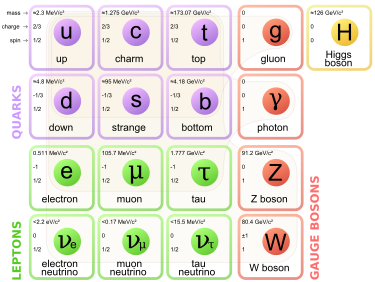
\includegraphics[width=0.4\textwidth]{./Capitulos/StateArt/standard_model} 
 \label{Estandar model}
 \end{figure} 

Figure \ref{Estandar model} brings together the particles of the SM and specifies their properties. Fermions are grouped into three generations, each having two quarks and two leptons. Each member of a higher generation has a greater mass than the corresponding particle of the previous generation. The classification for quarks is the following: the first generation includes up and down quarks, the second generation strange and charm quarks, and the third generation bottom and top quarks. Each generation contains one quark with charge -1/3 (down-type) and other with charge +2/3 (up-type). For leptons, each generation includes one with -1 charge lepton and one neutral lepton (called neutrino) related to the correspond partner. Their classification is: first generation contains electron and electron neutrino, second muon and muon neutrino, and third tau and tau neutrino. The SM also postulates that for each known particle there exists another particle with the same value of mass and spin but opposite electric charge and different color charge. This partner is called antiparticle.

Additionally, according to the SM, the fundamental particles acquire their mass through their interaction with a scalar field denominated Higgs field. The mediating particle of this field is the Higgs boson and it was discovered on 2012 as announced by the experiments CMS and ATLAS. As it was mentioned earlier, SM is not a complete theory since there are physical phenomena that this theory does not explain. For example, it predicts neutrinos have zero mass but the observations neutrino oscillations indicate the opposite. Moreover, the SM does not provide a possible candidate for DM and does not explain the asymmetry of the neutrinos helicity. For this reason, some theories that extend the reach of SM have been proposed. One simple extension of SM that can explain the smallness of neutrino masses is Type I Seesaw mechanism. 

\section{Neutrinos in the Standard Model}

As it was mentioned earlier, the SM does not explain the reason why the mass of neutrinos is a factor of almost $10^{-6}$ smaller that the mass of the other fermions. Moreover the SM predicts that
the mass of the neutrinos is zero. Addiotionally, it does not provide an explanation to the fact that only left-handed neutrinos have been observed in nature. 
In this section we are going to work on possible solutions to these problems. \footnote{The detailed calculations of the theory explained here are stated in \ref{apendice_neutrinos}}

\subsection{Dirac Mass}

First, we start by studying the Dirac mass term of a free fermion. The Lagrangian equation for a fermion particle is given by the expression:

\begin{equation}
 L = \overline{\psi} \left( i \gamma ^\mu \partial_{\mu} - m \right) \psi \text{,}
\end{equation}

where $\psi$ is the Dirac Spinor. From this Lagrangian expression it is possible to see that in the SM the mass is included through the second term in the equation which is called ``Dirac mass term'':

\begin{equation}
 m \overline{\psi} \psi
\end{equation}

We can write the Dirac Spinor as a sum of its left- and right- chiral states:

\begin{equation}\label{Dirac mass term}
 m \overline{\psi} \psi = m \left( \overbar{\psi_L + \psi_R} \right) \left( \psi_L + \psi_R \right) = m \overline{\psi_L} \psi_R + m \overline{\psi_R}\psi_L
\end{equation} 

In the last expression we used the fact that: $\overline{\psi_L}\psi_L = \overline{\psi_R}\psi_R = 0$ which is proved in Appedix \ref{apendice_neutrinos}. It can be seen from Equation \ref{Dirac mass term} that a massive particle must have both quiral states: left and right. Thus, the Dirac mass can be interpreted as the coupling constant between the two chiral states. Since right-handed 
neutrinos had been never observed in nature, it is expected that neutrinos have zero mass. Although, experiments of neutrino oscillations indicate that neutrinos have a small mass of 
the order of MeV. The former implies either the existence of a right-handed neutrino which is responsible for the mass of the neutrino, or that there exists other sort of mass term \cite{Theory_neutrinos}.

\subsection{Majorana Mass}

The Majorana Mechanism is based on expressing the mass term in the Lagrangian in only the left-handed chiral state terms.
To do this we start by decomposing the wavefunction into its left and right chiral states in the Dirac Lagrangian \cite{Theory_neutrinos_book} :

\begin{align}
  \phantom{i = j = k}
  &\begin{aligned}
    \mathllap{L} &= \overline{\psi} \left( i \gamma ^\mu \partial_{\mu} - m \right) \psi \\
    \mathllap{}  &= (\overline{\psi_L} + \overline{\psi_R})( i \gamma ^\mu \partial_{\mu} - m)(\psi_L + \psi_R) \\
     \mathllap{} &= i \overline{\psi_L}\gamma^\mu\partial_\mu \psi_L - \overline{\psi_L} m \psi_R +
     i\overline{\psi_R}\gamma^\mu \partial_\mu \psi_R - \overline{\psi_R}m\psi_L
   &\end{aligned}
\end{align}

Since $\overline{\psi_L}\psi_L = \overline{\psi_R}\psi_R = 0$ and $\overline{\psi_R}\gamma^\mu \partial_\mu \psi_L = \overline{\psi_L}\gamma^\mu\partial_\mu \psi_R = 0$
as it is explained in the Appendix \ref{apendice_neutrinos}. Now, we can replace the expression of this Lagrangian in the Euler-Lagrange equation:

\begin{equation}
\frac{\partial L}{\partial (\partial \phi)} - \frac{\partial L}{\partial \phi} = 0
\end{equation}

By doing this we find that the two equations of motion for the fields are two coupled Dirac equations for the right- and left- handed fields:

\begin{equation}\label{majorana_objetive}
i \gamma ^\mu \partial_\mu \psi_L = m \psi_R
\end{equation} 
\begin{equation}\label{majorana_start}
i \gamma ^\mu \partial_\mu \psi_R = m \psi_L
\end{equation} 

In the formulation of the SM the mass of the neutrino is zero, in this case we obtain two equations which are called ``Weyl equations'':
\begin{equation}
i \gamma ^\mu \partial_\mu \psi_L = 0
\end{equation}
\begin{equation}
i \gamma ^\mu \partial_\mu \psi_R = 0
\end{equation}

The former means that neutrinos can be described using two two-component spinors that are helicity eigenstates. These eigenstates represent two states 
with definite and opposite helicity which correspond to the left- and right-handed neutrinos. However, since we have not observed a right-handed neutrino 
we just represent the neutrino as a single left-handed massless field \cite{Theory_neutrinos}.

Majorana worked out a way to describe a massive neutrino just in terms of it's left-handed field.
This calculation is performed in the Appendix \ref{apendice_neutrinos}. The objective of Majorana was to write the Equation
\ref{majorana_start} as \ref{majorana_objetive} by finding an expression for $\psi_R$ in terms of $\psi_L$. By doing some manipulations of the Equation \ref{majorana_start} we 
find that it can be written as:  

\begin{equation} \label{Equation_not_used}
i \gamma^\mu \partial_\mu C \overline{\psi}^\intercal_R = m C \overline{\psi}^{\intercal}_L \text{,}
\end{equation}

where $C$ is the operator charge conjugation operator. Now, the Equation \ref{Equation_not_used} would have the same structure
as Equation \ref{majorana_objetive} if the right-handed term is imposed to be:

\begin{equation} 
\label{Expression_right_handed}
\psi_R = C \overline{\psi}^\intercal_L
\end{equation}

The former assumption requires $C \overline{\psi}^\intercal_L$ to be right-handed, this is proved in the Appendix \ref{apendice_neutrinos}. Thus, the complete Majorana 
field can be written as:
\begin{equation}
\psi = \psi_L + \psi_R = \psi_L + C \overline{\psi}^\intercal_L
\end{equation}

Defining the charge-conjugate field as: $\psi^C_L = C \overline{\psi}^\intercal_L$, we get for the expression of the complete Majorana field:

\begin{equation} \label{Structure_imposed}
\psi = \psi_L + \psi^C_L
\end{equation}

The implications of requiring the right-handed component of $\psi$ to satisfy the Equation                                                    \ref{Structure_imposed} can be studied by taking the charge conjugate of the complete Majorana field. 

\begin{equation}
\psi^C = (\psi_L + \psi^C_L)^C = \psi^C_L + \psi_L = \psi
\end{equation}

Having in mind that the charge conjugation operator turns a particle state into an antiparticle state, it can be deduced that a Majorana particle is its own antiparticle.
Since the charge conjugation operator flips the sign of electric charge, a Majorana particle must be neutral. Thus, the neutrino is the only fermion that could be a Majorana particle.

\subsubsection{Majorana Mass Term}

In Equation \ref{Dirac mass term} we saw that the mass term in the Lagrangian couples the left and right chiral states of the neutrino. Replacing the 
expression we found in Equation \ref{Expression_right_handed} for the right-handed component of the neutrino field in the mass term of the Lagrangian we get the equation \ref{majorana_mass_term} \cite{Theory_neutrinos_book}. In this equation we denoted the Dirac Spinor of neutrino as $\nu$. Having in mind that the hermitian conjugated of the first term in the equation is identical, we normalize the Lagrangian and obtain:

%EXPLICAAAAAR expresion y 1/2

\begin{equation}\label{majorana_mass_term}
L_{Maj}^{L} = m \overline{\nu_L} \nu_L^C + m \overline{\nu_L^C} \nu_L = \frac{1}{2} m \overline{\nu_L^{C}} \nu_L
\end{equation}

%EXPLICAR LEPTON NUMBER VIOLATION

\section{Seesaw Mechanism}

As it was mentioned before, in the case that the right-handed chiral field does not exist there can be no Dirac mass term. However, we can have a Majarona mass term in the 
Lagrangian (associated to a left-handed quiral field) so the neutrino would be a Majorana particle:

\begin{equation}
L_{Maj}^{L} = \frac{1}{2} m_L \overline{\nu^{C}}_L \nu_L
\end{equation}

%The term $m_L$ is forbidden by electroweak symmetry and it appears after its spontaneous breakdown through the Higgs Mechanism, hence such a term can not exist.
In order to let the neutrino to have mass, a right-handed neutrino that interacts only with gravity and the Higgs field must exist.
%EXPLICARRRRRRRRRRRRRRRRRRRRRRRRRRRRRRRRRRRRRRRRRRRRRRRRRR
If we consider that a right-handed chiral neutrino can exist, we would have to add different terms to the Lagrangian. First, if 
we assume that it is possible to write a left-handed Majorana field, we have for the first term:

\begin{equation}
L_L^{M} = m_L \overline{\nu_L} \nu_{L}^C + m_L \overline{\nu_L^C} \nu_L
\end{equation}

Additionally, we have to include a similar term which is the right-handed Majorana field:

\begin{equation}
L_R^{M} = m_R \overline{\nu_R^C} \nu_{R} + m_R \overline{\nu_R} \nu_R^C
\end{equation}

We also have to add Dirac mass terms in order to study the most general Lagrangian: the first Dirac mass term we mentioned on this section (Equation \ref{Dirac normal}) and another one that comes from the 
charge-conjugate fields (Equation \ref{Dirac conjugated}) \cite{Theory_neutrinos}:

\begin{equation}\label{Dirac normal}
L = m_D \overline{\nu_L}\nu_R + m_D \overline{\nu_R}\nu_L
\end{equation} 

\begin{equation}\label{Dirac conjugated}
L = m_D \overline{\nu_R^C} \nu_L^C + m_D \overline{\nu_L^C}\nu_R^C
\end{equation} 

Since the hermitian conjugate of each equation is identical, we can write the most general mass term as a sum ot the Lagrangians we just mentioned:
\begin{equation}
L = \frac{1}{2} \left( m_L \overline{\nu_L^C} \nu_L + m_R \overline{\nu_R^C} \nu_{R} + m_D \overline{\nu_R}\nu_L + m_D \overline{\nu_L^C}\nu_R^C   \right)
\end{equation}

The former equation can be written as a matrix equation: 

\begin{equation}\label{matrix_m_sa}
L_{mass} \propto
\begin{pmatrix} 
  \overline{\nu_L^C} & \overline{\nu_R}
\end{pmatrix}
\begin{pmatrix}
  m_L & m_D \\
  m_D & m_R  
\end{pmatrix}
\begin{pmatrix}
  \nu_L \\
  \nu_R^C  
\end{pmatrix}
\end{equation}

Equation \ref{matrix_m_sa} expresses the Lagrangian in terms of the left and right chiral states. These states do not have a definite mass because the matrix is not diagonal. 
Thus, the left and right chiral states do not correspond to the physical particles (which have a definite mass). Instead the real particles are a superposition of the 
mass eigenstates. In order to find the mass eigenvalues we need to diagonalize the M matrix (the one in the middle of the former equation). This calculation is 
explained in Appendix \ref{apendice_neutrinos}. We find the mass eigenstates are given by the expression:

\begin{equation}
m_{1,2} = \frac{1}{2} \left[ (m_L + m_R) \pm \sqrt{(m_L - m_R)^2 + 4m_D^2} \right]
\end{equation}
 
The fact that the SM does not allow a Majorana left-chiral mass term implies $m_L = 0$. Next, we are going to study the expression of the mass eigenstates $m_1$ and $m_2$. 
When we choose $m_R >> m_D$, we get for the mass eigenvalues:

\begin{equation}
m_1 = \frac{m_D^2}{m_R}
\end{equation}

\begin{equation}
m_2 = m_R \left( 1 + \frac{m_D^2}{m_R^2}\right) \approx m_R 
\end{equation}
 
From both equations above we can deduce that if there a neutrino with mass $m_2$ very large exists, then the other neutrino must have a small mass. 
The former fact is the reason why this mechanism is called ``Seesaw'': the mass of each physical neutrino is controlled by the mass eigenvalues in a way such that when one neutrino is light
the other is heavier \cite{Theory_neutrinos_book}. Now, the neutrino mass eigenstates are given by the following expresions:

\begin{equation}
\label{nu_1}
\nu_1 \propto \left( \nu_L + \nu_L^C \right) - \frac{m_D}{m_R^2} \left( \nu_R + \nu_R^C \right)
\end{equation}

\begin{equation}
\label{nu_2}
\nu_2 \propto \left( \nu_R + \nu_R^C \right) + \frac{m_D}{m_R^2} \left( \nu_L + \nu_L^C \right)
\end{equation}

The Equations \ref{nu_1} and \ref{nu_2} show that $\nu_1$ is mostly the left-handed light Majorana neutrino while $\nu_2$ is the heavy sterile right-handed neutrino. This is the explanation 
that the Seesaw Mechanism gives to the fact that the neutrino is much lighter than the other fermions. 
 
 
 
 
 
 
%\thispagestyle{empty}
 \chapter{Important Concepts and Variable Definitions}
 
 \section{Jets}
 A Jet can be defined as a high energy shower of stable particles that comes from fragmentation of quarks or gluons. The initial quarks and gluons in the process are know ``initial partons''.
 Due to the initial partons are colour charged, they can not be isolated singularly (this phenomenon is called ``colour confinement''. Since it is not possible for charged particles to be isolated 
 they must go through a non-perturvative process that converts them into colour neutral particles. This process is called ``hadronization'' and there are different models to explain it. According to 
 the string model, the confining nature of strong interaction increases the potential colour in a proportional way as the distance between the initial partons. When the distance reaches a certain 
 critical value it is energetically favourable to produce a quark pair from the vacuum. Finally, by this proccess the inital colour charged particles are convert into bound colour-singlet hadronic 
 states. \\
 %Citar libro: Particle detectors Calus GRupen and Boris shwartz
 
 Besides jets may display a structure with properties that could indicate which were the initial partons interacting, they are hard to study individually when there is a numerous quantity of them
 in an event. The former is because it is almost imposible to attach all particles in an event final state to a single initial parton. The reconstruction of jets depends of elements like the 
 fragmentation process, detectors effects, among others. Thus, there exist algorithms which cluster some particles in a final state so that it is possible to determine properties as 4-momentum 
 and jet shapes. The objetive of this algorithms is to determine the inital interacting partons and approximate its directions and energies. \\
 
 According to the reconstruction algorithms we can define a jet at three different levels. At partonic level a jet can be understood as a quark or a gluon. At hadronic level can be referred to the
 hadrons produced due to the hadronization process. Finally, at a detector level can be understood as a the tracks detected and the energy deposited in the calorimeters of the detector. The 
 reconstuction algorithms that are going to be used for this analysis consist in enclose in cones the regions where there is a numerous detection of particles. 
 %Citar tesis Luis Alfredo
 
 \section{Cross Section and Luminosity}
 
 In High Energy Physics the cross section $\sigma$ concept is the probability that a certain event of interest has to occur. This quantity is proportional to the energy of the event production. The unit 
 used for cross sections is the bar (1 b = $10^{-28} m^2$). The number of a certain interaction in a fixed target experiment is proportional to its cross section, the particles flux, and the
 number of atoms per cubic meter in the target multiplied by the lenght. The inverse of the last quantity is called ``target constant $F$'' and it has the dimesion of an area. Thus, it is possible
 to make an estimation of the number of interactions per second using:
 
 %citar libro data analysis techniques for high energy physics
 \begin{equation}
  \frac{N_{events}}{s} = \sigma \frac{N_{flux}/s}{F} = \sigma \times Luminosity
 \end{equation}

 In the last identity we defined the concept of luminosity, which is a measure of sensitivity and depends on the energy and on the beam dynamics.  The luminosity is a quantity that is used to 
 describe the performance of a particle accelerator. It has units of the inverse of cross section, which is know as inverse barns $fb^{-1}$ and it is equivalent to $(1 fb = 10^{-28} m^2)$. 
 In particle colliders the 
 luminosity depends of different as the number of particles per bunch $N_b$, the number of bunches in each beam $\kappa_b$, the revolution frequency $f$ at the storage ring and the beam radii 
 $ \sigma$ of the bunches at the crossing point:
 
 \begin{equation}
  L = \frac{N_b^2 f \kappa_b}{4\pi \sigma^2} 
 \end{equation}

 \section{Pseudorapidity}
 
 The variable Pseudorapidity is defined as a parametrization of the CMS detector coordinates. These coordinates are ilustrated in the figure \ref{CMSCoordinates}:
 
 %\graphicspath{./Capitulos/VariableDefinitions}
 
 \begin{figure}[h] \label{CMSCoordinates}
 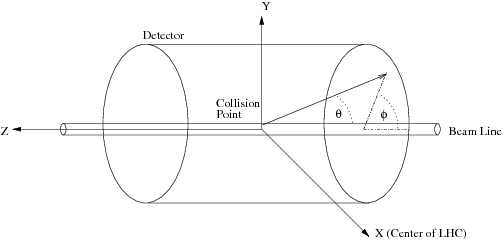
\includegraphics[width=0.75\textwidth]{./Capitulos/VariableDefinitions/CMS_coordinates}  
  \caption{CMS detector coordinates}
 \end{figure}

The origen of the CMS coordinates coincides with the point in which a collision occurs in the detector. 
The polar angle is described by the parameter $\theta$ and it is measured with respect to the z axis.
The azimuthal angle is denoted by $\Phi$ and it is measured in the xy plane from the x axis. The Pseudorapidity is defined in terms of the polar angle as:

\begin{equation}
 \eta \equiv - \ln \left( \tan (\theta /2 ) \right)
\end{equation}

 The motivation to define and use this variable is that while $\Delta \theta$ is not a Lorentz invariant $\Delta \eta$ is. Moreover, the quantity of particles in function on the variable $\eta$
 is approximately uniform in a cilindrical detector. 
 
  
 \section{$p_T$ and $\vec{E_T^{miss}}$}

 The quantity $p_T$ is the transversal momentum and it is the projection of the linear momentum onto the xy plane. This variable is used instead of the linear momentum because the initial beams
 are moving just in the z axis (the initial momentum in the xy plane is zero), so when a collision is produced the interesant effects occur in the transverse plane.\\
 %the particles adquiere momentum in the xy plane. 
 
 As it was already mentioned the momentum in the tranverse plane is zero before the collision. Since the tranverse momentum has to be conserved, after the collision it must be zero. We can write
 the total momentum as the sum of the particles that are detected (visible particles) and the ones that are not detected (invisible particles), the former can be expressed as:
 
 \begin{equation}
  0 = \sum_{i=1}^N \vec{P_T(i)} = \sum_{j=1}^M \vec{P_T(j)}^{visibles} + \sum_{k=M}^{N-M} \vec{P_T(k)}^{invisibles}
 \end{equation}

 The former equation motivates the definition of a variable called ``Missing transverse energy'' ($\vec{E_T^{miss}}$), which is defined as the sum of the transverse momentum of the invisible
 particles:
 
 \begin{equation}
  \vec{E_T^{miss}} \equiv \sum_{k=M}^{N-M}\vec{P_T(k)}^{invisibles} = - \sum_{j=1}^M  \vec{P_T(j)}^{visibles}
 \end{equation}

 
 \section{Impact Parameter}
The vertex of a track is a variable of importance because it can be used to determine the position of the point of interaction and the momentum vector of the tracks emerging from the vertex. The 
vertex fit can also be used to check the association of tracks to a vertex, in oder words, to determine if a track actually originates from a certain vertex. In order to determine the direction of the
track connecting a primary and a secondary vertices we have to find the position of the secondary vertex.
It is relevant to find the position
of any secondary vertex since it can determine the direction of the track conneting both vertices.
 
 
 
 
 
 
 
 
 
 
 
 
 
 
 
 
 
 
 
 
 
 
 
\chapter{CMS Detector}

In this analysis we are going to perform simulations of collisions occurring at the CMS experiment, so we have to take into account the specific characteristics of this detector. For this reason
the components of the CMS are going to be explaind.
The CMS is one of the seven experiments located at the Large Hadron Collider (LHC), which is the largest and most powerfull particle accelerator in the world. This accelerator collides protons 
and heavy ions at very high energies of the order of 13 TeV and 6.37 TeV, respectively, with the objective of studying the elemental particles of the universe. 

%Energia ions http://accelconf.web.cern.ch/accelconf/ipac2016/papers/tupmw027.pdf

The LHC is conformed by a ring of almost 27 km of perimeter and by 7 detectors located at the different collision points of the ring. Two of these detector are general-purpose detectors, and they 
are referred as experiments CMS and ATLAS (A Toroidal LHC ApparatuS). Both experiments share the same goals of searching physics beyond the SM. The physics program includes measurements of the Higgs boson, 
Supersymmetry searches, dark matter, detection of extra dimensions, among others. The difference between both experiments is that they use different desings and software. In the ATLAS detector the 
magnetic field is produced by a central toroid, two end toroids and a central solenoid, while the CMS detector is built around a superconducting solenoid magnet.  

The CMS and ATLAS detectors have a cylindrical form in order to have the most uniform magnetic field posible. They are centered in the direction of the interacting beams and the collision point and have two ``end-caps'' to cover the forward regions. These detectors are conformed by the same general components, from the inner part of the detector to the outer part. These components are: a tracking system, an electromagnetic and a hadronic calorimeter, and muon detectors. They also have magnets to curve the path of the electric charged particles, so it can be determined whether a particle has a positive or negative charge. Aditionally, the measurement of the curve can be used to calculate the momentum of the charged particle. In Figure \ref{CMS_detector}, there is a diagram showing the structure of the CMS detector. This image also shows the interaction of different particles with the parts of the detector.

%\section{Accelarator and Storage Ring}

%CITAAAAAAAAAAAAAAAAAAAAAAAAAAR http://cms.web.cern.ch/news/detector-overview

 \begin{figure}[h]
 \centering
 \caption{CMS detector.}
 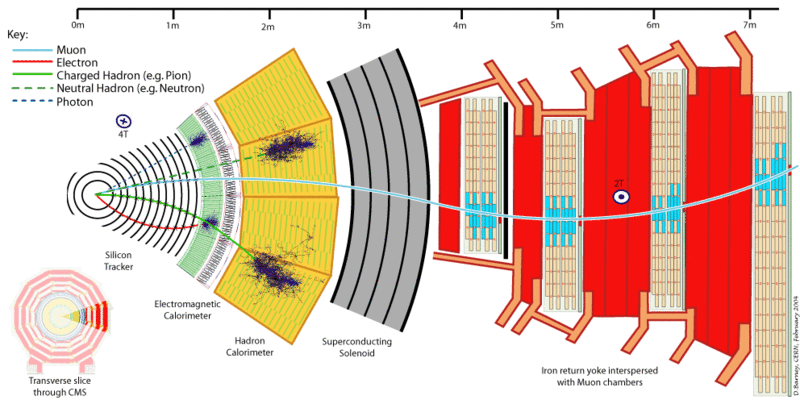
\includegraphics[width=0.9\textwidth]{./Capitulos/CMS/CMS}  
 \label{CMS_detector}
 \end{figure}

\section{Tracking System}

Since every 25 ns there is a collision at the center of the CMS detector and almost 1000 particles are going to be produced, it is necessary to have a tracking system able to record measurements 
of all the particles that are produced. This tracking system must be located the nearest possible to the region where the collision occurs. This tracking system is used to measure the momentum and 
vertices of the particles with a high precision. The inner detectors are built with silicon detectors, with high granularity pixel systems at the smallest radii, and silicon-strip detectors at 
larger ones. 
%Citar libro:perspectives on LHC Physics


The properties of the tracking system are: fast recording of measurements, toleration to high radiation doses, ensembled with light material and toleration of the severe conditions imposed by the low temperature at LHC (of almost 2 K). One of the major challenges for the inner dectector parts is the control of aging effects because the damage produced by irradiation is severe. The silicon detectors are p-n junction diodes, so when a particle crosses the detector, it causes the liberation of electron-hole pairs, which move to the electrodes of the system. The tracking system in the CMS detector covers the range within $|\eta|<2.5$, the region where most of the relevant particles for the analysis arrive. 

The flux of particles arriving to a point in the detector depends of the distance from the center of collision to where the detector is located: as the flux crosses the detector material the quantity of particles decreases. Thus, the resolution of the tracking system does not need to be so high in the intermediate and end caps regions. For this reason, in the first region of the tracking system (the closest to the interaction point), there are silicon pixel detectors with cell size of $100 \times 150 \mu \text{m}^2$. The innermost layer of pixels is located as near to the beam as it is practical, this is at a radius around 4.5 cm.
 
The silicon pixels are expensive and have high power density. Aditionally, the flux of particles at an intermediate region of the inner detectors is low enough to use silicon microstrips. Thus, in the region of radius greater that 20-55 cm the silicon pixels are replaced by silicon microstrips. These silicon microstrip are arranged in a special way to improve the resolution in the z axis. These barrel cylinders and end-caps disks, as the silicon pixels, cover the region of $|\eta| < 2.5$. The strip dimensions are or around $11 \text{cm} \times 100 \mu \text{m}$.

In the outermost region of the tracking system (at a radius greater that 55 cm) the particle flux is low enough to use larger-pitch silicon microstrips. The maximum size of these cells is $25\text{cm} \times 80 \mu \text{m}$. There are 6 layers of these silicon microstrips modules in the barrel and 9 end-caps disks that also cover the region given by $|\eta|< 2.5$.

%Escribir interaccion particulas con tracking systems

\section{Calorimetry}

Surrounding the tracking system of the CMS detector are located the electromagnetic and hadronic calorimeters. The calorimeters measure the energy of the incoming particles, by absorbing the particles and transforming them into heat. The priorities of the electromagnetic calorimeter is to measure precisely the energy of electrons and photons, to make measurements of their position and direction of movement. The priorities of the hadronic calorimeter are to make precise measurements of the jets energy and to cover a larger area of $|\eta| < 5$. The area covered has to be large with the purpose of attributing all the $\vec{E}_T^{miss}$ to the particles that cannot be detected.

The electromagnetic and hadron calorimeters are made out of scintillation crystals. When a high energy particle goes through the detector, it collides with the nuclei of the material and generates a shower of particles. The product particles of this interaction excite the atoms in the material by making the electrons in the material go to a higher orbit. When each electron returns to the initial orbit, it emits a photon. 

Then, the light emmited by the scintillator is measured by photodiodes, which have the function of converting the optical signals into electronic signals. The photodiodes mechanism is based on the photoelectric effect: the photons emmited by the scintillator arrive to the light-sensitive area of the photodiode and expulse electrons in this surface. Then these electrons are accelerated and strike a silicon diode target, which causes that more electrons get expelled of this surface. At the end, one obtains an amplification of the initial signal which is measured.

\subsection{Electromagnetic Calorimeter}

The electromagnetic calorimeter is an entirely active homogeneus calorimeter made of lead tungstate (PbWO$_4$) crystal. It has 61,200 crystal in the central barrel part and 7,324  in each of the two end-caps. As a consequence from the use of high density crystals, the calorimeter is fast, has fine granularity and is radiation resistant. 

The lead tungstate crystal material was chosen for different reasons. First, it emits a short radiation length which is easy to record. Second, it has small Moliere radius, which is defined as the radius of the cylinder surrouding the 90\% of the shower's energy deposition. That leads to a compact calorimeter in size. Third, the lead tungstate crystal has short decay time constant, which allows the calorimeter to have a fast response. Lastly, it is resistant to high dosis of radiation. Moreover, due to the electromagnetic calorimeter is located within the solenoid, avalanche photodiodes are used as photodetector because they can operate under the magnetic field of 4T. 

\subsection{Hadron Calorimeter}

Surrouding the electromagnetic calorimeter is located the hadron calorimeter. Its objetive is to measure the energy and direction of jets. It is designed to detect the most possible particles product of a collision, so it is said that the detector has a hermetic coverage. The priority of this calorimeter is to determine as correct as possible the missing transverse energy ($\vec{E_T^{miss}}$). The hadron calorimeter is made out of plastic scintillator tiles with wavelenght-shifting fiber. The wavelength-shifting is used to shift the wavelenght of the light emitted by the scintillator in a the range in which the efficency of the photodiodes is high.

The hadron calorimeter is restricted to fill the area between the outer cap of the electronic calorimeter and the magnet coil, this is $1.77 \text{m} < R < 2.95\text{m}$. The layers of the scintillator tiles are alternately placed with layers of copper in the barrel to form the hadron calorimeter. The end-caps of the calorimeter covers the area of pseudorapidity given by $|\eta|= 3$ and $|\eta|= 5$.


\section{Muon Detector}

The muon system detector consists of several multi-layer large area gas-based detectors. The main objetive of this detector is to take precise measurements of muon tracks. Since the muon system detector is located at the outermost part of the CMS the radiation level is receives is very low in comparison to the tracking system and the calorimeters. The CMS muon detector has three tasks: identify the muon particles, measure its momentum and triggering on them (this concept is explained in the next subchapter). The layers of the muon detector alternate with layers of the yoke where the magnetic field returns, which is called flux-return yoke. 

The flux-return yoke curves the path of the particles in the opposite direction as it was inside the copper layers. It also can be used for good resolution muon identification because it absorbs some hadrons with low energy. The high magnetic field applied and the flux-return yoke allows to take precise measurements of the muon momentum. The muon system detector surrounds the hadron  calorimeter and, consists also of a barrel section and two end-caps. 

The CMS detector has three types of gaseous particle detectors for muon measurements. In the barrel region where the neutron-induced background is low and the magnetic field is almost uniform, there are located drift chambers. The drift chambers are tubes each of 4 cm wide that contain a strechted wire immersed in a gas. When a muon crosses the chamber it hits the electrons of the atoms in the gas. Then, the free electrons arrive to the positive charged wire and it is measured an electronic signal. By measuring the time it takes for an electron to arrive to the cathode (known as drift-time) and the velocity of the free electrons (drift velocity) it is possible to determine the position of the initial muon. The drift chambers cover the region of pseudorapidity given by $\eta < 1.2$.
%Referenciaaaaaaaaaaa: http://cms.web.cern.ch/news/muon-drift-tubes
%REferenciaaaaaaaaaaaa: Claus gruppen - Particle detectors 
  
In the two-end caps regions there are cathode strip chambers (CSC). In these regions the muon rates and backgrounds levels are high and the magnetic field is large and non-uniform. The CSC uses the
same principle as the drift chamber to measure the position of muons. The difference is that the CSC consist of anode wires crossed with cathode strips, these arrays are also immersed in a gas. When
a charge particle crosses the detector, it hits the atoms of the gas expelling electrons. The free electrons are guided by the electric field and arrive to the anode wires, while the positive ions 
move towards the cathode. The CSC have fast response time, fine sementation and are radiation resistant. Thus they are able to take precise measurements of time and position. These detectors cover the
area given by $|\eta| < 2.4$. Due to the fact that the tracking system and muon detectors take indepedent measurements of the muon momentum, it is possible to find errors and check both measurements.

%http://cms.web.cern.ch/news/cathode-strip-chambers

An additional redundacy in the muon measurements is contributed by resistive plate chambers (RPC) in the barrel and the two end-caps regions. It is similar to the other two muons detectors: it is 
conformed by two plates, one is the cathode and the other the anode and these plates are separated by a gas. When a charged particle crosses the detector, the resulting free electrons move to the anode.
The electric signal is received by metallic strips after a precise time delay. The set of hit strips gives a precise measurement of the muon position and momentum.
%http://cms.web.cern.ch/news/resistive-plate-chambers

\section{Triggers}

Since at the LHC the there are bunch crossings every by 25 ns with a peak crossing rate of 31.6 MHz, nearly a billion proton-proton events are produced every second. Thus, it is necessary to decide
to store or not store an event in order to reduce the computational resources use. Triggers have the task of applying a primary selection on the data at real-time. The triggers take the data and quickly 
decide which events that are interesting pass to the next phase of filtering. The triggers need to have a rejection factor of almost $10^7$. As a consequence, it allows to store just around 100-200 
carefully selected events per second to be proccessed later. 

The first triggering level uses a partial amount of the total information given by the detector and takes decisions in less that 3.2 ns. 
It reduces the data rate to nearly 100 kHz. High level triggers use a network of thousands of processors and fast switches. They get the information gradually and use algorithms in order to reduce 
the amount of data. The final product is that at a rate of 150-200 Hz each event occupies around 1.5 Mb. The former leads to the LHC to have an annual data volume of around 10 PB . After an event 
passes the first triggering level, the resulting data is transferred from the detector electronics into readout buffers. Then, the signal is processed and compressed while the events are studied by 
processors with several thousands of central processing units. The event then is directed to a single processor with the objective of performing detailed calculations of the critical parameters of the 
event and reduce the amount of data.

%https://lhc-machine-outreach.web.cern.ch/lhc-machine-outreach/collisions.htm






%\thispagestyle{empty}
 \chapter{Model and backgrounds}

 
\section{Signal of Interest}

The model that was studied is based on a recently proposed new mechanism of production of heavy neutrinos through the Higgs Boson decay \cite{Seesaw Mechanism with displaced vertices}. One
favourable characteristic of this model is that in a natural scenario the mass of the heavy neutrinos can lie at the electroweak scale. The theoretical study by \cite{Seesaw Mechanism with displaced vertices} 
proposes the experimental search of the heavy neutrinos using a technique known as displaced vertices.

According to this model, when the mass of the heavy neutrinos is inferior than the mass of the Higgs, the latter can present novel decay channels. The Higgs boson can decay into a light and a heavy
neutrino, followed by a subsequent decay of the heavy neutrino via a charged or neutral current interaction. Then, the decays of the heavy neutrino can be represented by: $N \rightarrow l^+ l^- \nu$
or $N \rightarrow l q q'$. Thus, there are two possible final states of the event of interest: two leptons, two jets (from the VBF process) and $\vec{E_T^{miss}}$ (due to the neutrino) or four jets 
(two of the VBF process and two from the quarks of the heavy neutrino decays), $\vec{E_T^{miss}}$ and one lepton. The first type of final state is going to be called leptonic signal, while the second
will be named hadronic signal.

If the heavy neutrino has a mass of the order of a few GeV, the Higgs and heavy neutrino would travel a certain distance before decaying. Since both particles are not detected, the decay products are expected to have associated tracks with displaced vertices. For this reason, the presence of displaced vertices in the detector is an important signal to prove this model because it could indicates the presence of the heavy neutrino in the detector. Nevertheless, in this model the resulting leptons have a low momentum. Thus, due to experimental restrictions of the available triggers in CMS and ATLAS, the theoretical analysis proposed in reference \cite{Seesaw Mechanism with displace vertices} is not achievable.  

The High Energy Physics Group at Universidad de los Andes has proposed a technique that allows to study at the LHC the production of heavy neutrinos through the decay of the Higgs boson. While in the model proposed in \cite{Seesaw Mechanism with displace vertices} considers the production of the Higgs boson through the fusion of two gluons, we consider the Higgs production through the fusion of two vector bosons. These vector bosons ($W^{\pm},Z^0,\gamma$) come from an interaction process between two quarks. Both quarks belong to protons from opposite beams that will collide in a particle accelerator. The former described process is know as Vector Boson Fusion (VBF) \cite{VBF processes}. 

Finally, as a result of the fusion of the two vector bosons, a Higgs boson is produced and the initial quarks that interacted manifest themselves as jets with high transverse momentum in opposite
hemispheres of the detector. For this reason, in Experimental Particle Collider Physics the events in which two jets of high transverse momentum are detected in opposite hemispheres of the detector 
and with a high separation of pseudorapidity are labeled as candidates of processes of VBF. The Feynman diagrams illustrating the processes already described is shown in Figure \ref{signals}, where \ref{signal_hadron_feynman} is the hadronic signal and \ref{signal_leptonic_feynman} illustrates the leptonic signal.

%CORREGIR IMAGENEEEEEEEEEEEEEEEEEEEEEEEEEEEEEEEES

\begin{figure}[h]
\centering
\begin{subfigure}{.5\textwidth}
  \centering
  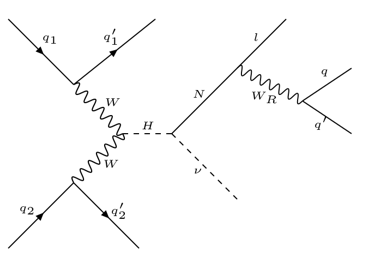
\includegraphics[width=1\linewidth]{./Capitulos/Model/hadron_signal}
  \caption{Feynman diagram for the hadron signal}
  \label{signal_hadron_feynman}
\end{subfigure}%
\begin{subfigure}{.5\textwidth}
  \centering
  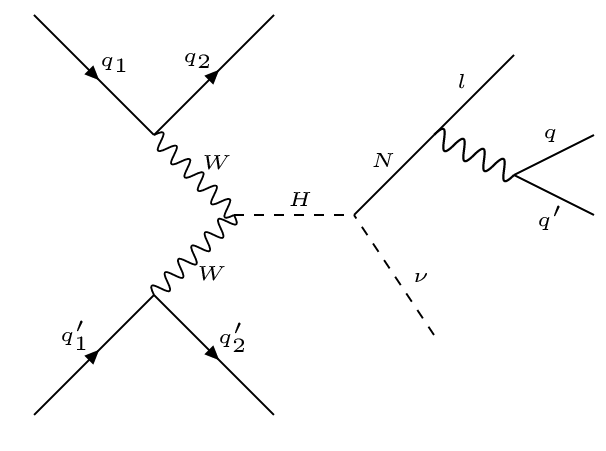
\includegraphics[width=1\linewidth]{./Capitulos/Model/leptonic_signal}
  \caption{Feynman diagram for the leptonic signal}
  \label{signal_leptonic_feynman}
\end{subfigure}
\caption{}
\label{signals}
\end{figure}


%The observation of the Higgs decay into heavy neutrinos would be a firm prove of the Type I Seesaw mechanism \cite{Type I Seesaw Mechanism}. The former would prove the existence of physics beyond the SM associated to the mass of the neutrinos.
 
 
 \section{Backgrounds}
 
The main problem of detecting an event of interest is that the magnitude of its signal is significantly smaller with respect to some other processes from the SM. For this reason, the processes from the
SM that have the same or similar final states as the signal are called backgrounds. Thus, it is fundamental to develop procedures in order to reduce the experimental background under the magnitude 
of the searched signal. These procedures usually use different variables (like the ones explain in the chapter \ref{Important_concepts_chapter}) that exploit the topology of the event and its 
kinematic characteristics. When a set of variables that separate the signal from the background is found, it is necessary to find the optimal values of them that allow to reduce as much as possible 
the background. 
 
The signal of interest that was described had two possible final states. For the hadronic signal: two leptons, two jets and $\vec{E_T^{miss}}$ and for the leptonic signal: four jets, 
$\vec{E_T^{miss}}$, and one lepton. Thus, the main backgrounds of the signal that have a similar final state are the W+jets background and the DY+jets background. In a inferior magnitude there
is other background that comes from the top pair production, referred as $t\overline{t}$.

 
\subsection{W+Jets Background}
  
%ASOCCIATEEEEEEEEEEED JEEEEEEEEEEEEEEEEETS  
The events in which is produced a W boson with jets has a large probabibity to occur in the collisions at the LHC. The W decay determines the final state of this event. Most of the times the W boson
has a hadronic decay and the other times have a leptonic decay. In leptonic decays, the W boson desintegrates into a lepton and a neutrino. Sometimes, in these events the particles 
comming from the interaction of the initial hadrons can produce a spontaneous radiative emission, which then is detected as a jet. It is said that this kind of jet comes from an Initial State 
Radiation (ISR). Thus, when the boson W decays leptonically, the final state is conformed by a lepton, $\vec{E_T^{miss}}$ (comming from the neutrino) and jets from ISR. The Feynman diagram is shown 
in Figure \ref{w_jets_feynman}.
  
%INCLUIR FRACCIONES PRECISAS DECAIMIENTOOOOOOOOOOOOOOO
  
 \begin{figure}[h] 
 \centering
 \caption{Feynman diagram for the W+jets Background}
 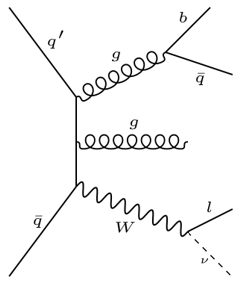
\includegraphics[width=0.4\textwidth]{./Capitulos/Model/w+jets}  
 \label{w_jets_feynman}
 \end{figure}  

 \subsection{Drell Yan + Jets Background}
 
 Other background for our signal of interest comes from the Drell Yan procces. In this process a quark and an antiquark comming from the initial interacting hadrons annihilate each other and this
 produce a virtual photon or a Z boson. The concept virtual photon means that this particle is created for a very short period of time. We studied this process only when the Z boson decays into a 
 pair lepton-antilepton, because in this case the final state is the most similar to the one of the signal. Specifically, we considered the events were the Z decays into a pair 
 tau and antitau ($\tau \overline{\tau}$). This process was simulated with the presence of a jet from ISR. Thus, the final state is conformed by one tau, jets (from the ISR procces), 
 $\vec{E_T^{miss}}$ (from the erroneus identification of the one of the taus). The Figure \ref{dy_jets_feynman} shows the Feynman diagram for this process.
 
  \begin{figure}[h] 
 \centering
 \caption{Feynman diagram for the DY+jets Background}
 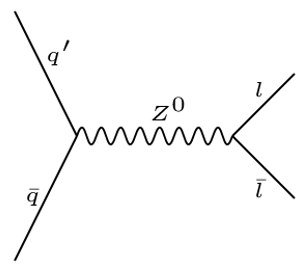
\includegraphics[width=0.4\textwidth]{./Capitulos/Model/DY+jets} 
 \label{dy_jets_feynman}
 \end{figure} 
 
 \subsection{$t \overline{t}$ Background}
 
 Other background for our signal of interest is produced by the the top anti-top creation pair. These events are produced when a gluon commming from the interaction of two colliding protons decays into
 a pair top-antitop particles. A Feynman diagram for this background is showed in Figure \ref{t_tbar_feynman}. This figure shows that the final state of this event has three leptons, MET (comming
 from the neutrino) and one characteristic jet associated to the hadronization of a b quark. Since the signal do not have the presence of a quark b, this background can be strongly reduced by 
 making the filter of number of bjets equal to zero.
 
 %https://www-d0.fnal.gov/Run2Physics/top/top_public_web_pages/top_feynman_diagrams.html
 
  \begin{figure}[h] 
 \centering
 \caption{Feynman diagram for $t \overline{t}$ Background}
 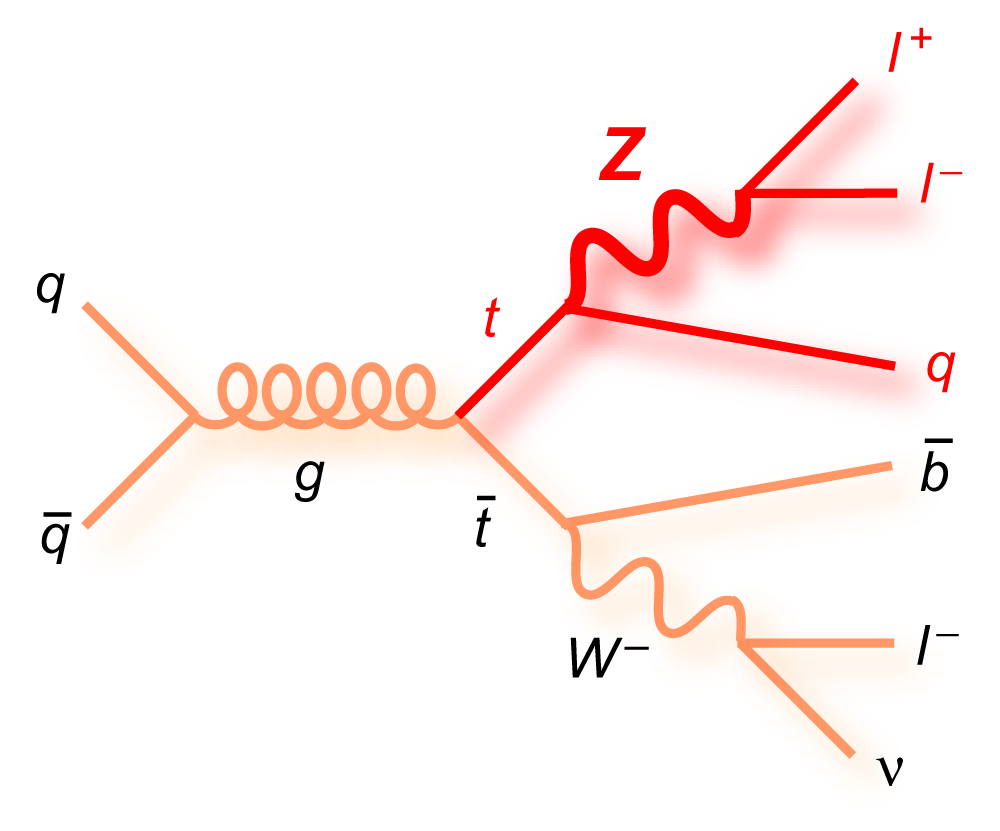
\includegraphics[width=0.4\textwidth]{./Capitulos/Model/t_tbar}  
 \label{t_tbar_feynman}
 \end{figure} 
 
 
 
 
 
%\thispagestyle{empty}
\chapter{Methodology} 

The objective of this project was to make a phenomenological study that allow the identification of a signal with the presence of a heavy neutrino in the experiments of the LHC. For this reason, 
the proposed methodology consisted in the use of different computational programs to simulate the signal and its background as it should be produced and measured at the CMS detector. Next, this data must go through a statistical analysis. The programs that were used to simulate the signal were MadGraph \cite{MadGraph 1, MadGraph 2} and Pythia \cite{Pythia}. Then, the program Delphes is used to simulate the behavior of the multi-purpose CMS detector \cite{Delphes}. Lastly, the statistical study of the data was developed with the software ROOT \cite{Root}, which determined the potential variables that could differentiate the signal and background. In the next paragraphs each program is going to be described, including the fundamental physical basis on which the program is constructed and its specific task in the development of the project.

\section{MadGraph}

The first program that was used is MadGraph, which is a generator of events that simulates the collisions of particle beams, which in our case are protons. MadGraph is written in Python programming language. The physical processes that MadGraph can simulate include processes from the SM and from physics beyond the SM that are based on certain theoretical models such as Supersymmetry. This program incorporates diverse physical parameters in order to include all the necessary elements to make phenomenological studies: it calculates the cross section of a certain event, it generates events with strong interactions (including possible decay of particles) and it offers relevant tools to manipulate the events and to make their posterior analysis. 

Madgraph uses perturbation theory to perform production calculations and to generate physical processes. The parameter entries are controlled in configuration files that are called input cards. 
These cards are use to modify essential variables in the production of the events, for example: the type of particles that will collide, the energy of the collision, number of events that are going to be simulated, mass of the generated particles, final states, among others. At the level of event generation it is possible to make basic cuts of minimal and maximal values of some kinematic variables. Moreover, the lastest version of MadGraph (MadGraph 5) has an useful characteristic: it can give an output file with matrix elements that can be used directly in the program Pythia. 

In order to produce an event of physics beyond the SM one has to describe the physical model in the form of a Lagrangian , a list of fields and parameters. Then use the former elements as parameters input of the MATEMATICA-based package FEYNRULES. Finally, FEYNRULES returns the Feynman rules corresponding to the Lagrangian of the model, which are used as input of MadGraph.


\section{Pythia}

The second computational program that was used is called Pythia. This program receives as parameter input the file generated by the software MadGraph. Pythia incorporates a set of physical models to develop the evolution of a few-body system into a complex multi-particle final state. Thus, the task of the Pythia in the project was to simulate the processes of hadronization of quarks and gluons.

%EXPANDIR MAAAAAAAAAAAAAAAAAAAAAAAAAAAAS

\section{Delphes}

The next program that was used receives as input the events produced by Pythia and it is called Delphes. This software makes a realistic simulation of the multipurpose CMS detector performance as it would happen if there was occurring such an event at CMS. The simulation includes a system of track reconstruction immersed in a magnetic field, an electromagnetic calorimeter, a hadronic calorimeter and a muon detection system.

Delphes takes into account the systematic errors that can be generated by the detector, which can be caused by multiple factors such as the resolution of the detectors. This program contemplates different characteristics of the event in the experiment: detector geometry, the track of the charged particles in the magnetic field, reconstruction of the events, and efficiencies of the reconstruction and particle identification. Due to that the proposed analysis includes the systematic errors that can be generated by the detector, it can be implemented in the experimental studies at the LHC. 

\section{ROOT}

The analysis of the simulated data was developed using the software ROOT. This software was created by the CERN laboratory. ROOT is written in the programming language C++ and it was 
designed to analyze data in particle physics. This program provides all the necessary tools to efficiently process large data, make statistical analyses, and visualize and store data. The program 
includes a numerous quantity of mathematical and statistic functions, numeric algorithms and methods for analysis of data regression. One key tool ROOT has are the histograms that can even use multidimensional data and estimate their density. The histograms can be manipulated, offer statistical information and can make data regression. 

The program ROOT receives as input parameter complementary information that allows it to do the best analysis of the signal: characteristics of the detector or configuration settings that were made in the simulations. ROOT includes other components like a command interpreter that makes quicker the analysis process and a graphic interface which contains a flexible set of tools. The former means that the set of tools can be modified using GUI Builder (the graphic interface constructor). This software can be used to analyse real or simulated data that have the same structure and consist of many events. 
%\thispagestyle{empty}
\chapter{Event Selection Criteria}
\label{Event_selection_criteria_chapter}

The analysis of the simulated data started by imposing a minimum value of 20.0 GeV on $p_T$ for b-jets and taus, and of 30.0 GeV on jets that are not associated to taus or b quarks. The low values 
required on $p_T$ are imposed in order to preselect the interesting particles. After this was done, we required a minimal distance of separation between taus and muons, taus and electrons, 
and taus and jets. The former was because we have to be sure that taus do not overlap with other objects, so the performed analysis can evade to commit errors such as tagging incorrectly a particle.
To do this, one has to impose a minimal value on the variable called minimal separation distance $\Delta R$, which is given by the Equation \ref{minimal_separation}. The minimal value imposed on this 
variable was 0.3 for taus with muons, electrons and jets. 

\begin{equation}
\Delta R \equiv \sqrt{\Delta \eta ^2 + \Delta \phi ^2}
\label{minimal_separation}
\end{equation}

Since we considered that the event of interest is generated by a procces of VBF, in the analysis was necessary to find the two possible jets that are related to the two VBF jets. This was done by 
searching two jets that satisfy the conditions of having a minimal value on $p_T$ of 50.0 GeV and $\eta$ greater that 5.0 each. The condition of minimal values on $p_T$ and $\eta$ is required 
because it is expected that the VBF jets have a large momentum and that they are located at the end-caps of the detector. Then, an algorithm was performed to select the pair of jets that have the 
largest sum of the mass of all possible combinations of jets pairs in each event. Finally, a minimal value of 100 GeV is required for the sum of the jets. That is how the two jets from the VBF 
process are determined. From both jets, the one with the hightest momentum is referred as the leading jet, and the other is know as the subleading jet. The required values to identify the VBF 
jets are part of the preselection process.

After the former preselection process is made, we have to find the minimal or maximum values of variables that allow to reduce the background of the signal at maximum. These minimal and maximum
required values are known as cuts. The first cut imposed in the analysis was on the number of jets. It was required a maximum number of 5 jets because the signal is expected to have 4 jets. An
additional jet is included in order to find the best two VBF jets. The second cut imposed was the presence of just one tau, due to the fact that this is a characteristic expected for the hadronic 
signal. 

Next, the third cut is imposed by requiring the number of b-jets to be zero. The former is done to reduce drastically the $t\overline{t}$ background because it has in the final state b-jets. The 
following cut made was on the variable $\vec{E_T^{miss}}$: it was required a value greater that 20 MeV. The former is because in the hadronic signal the neutrino is the only source of 
$\vec{E_T^{miss}}$, thus it is expected that this variable has a low value for our signal. Then, it was permorfed a cut on the absolute value of $\eta$ of the tau of maximum 2.1. This value was 
chosen because the tracking detector covers the range of $|\eta|<2.5$. Since the reconstruction cones of the taus have a radius of around 0.4, one has to impose a maximum value on $|\eta|$ of 
maximum 2.5 - 0.4 = 2.1 so the reconstruction algorithms are correctly applied in the area covered by the track detector.
  
After it was imposed a cut on the $\vec{E}_T^{miss}$ variable, the cuts motivated by the VBF proccess were performed. The first cut guarantees that there are minimum two jets that sasisfy the 
condition on $p_T$ to be candidates of VBF jets. Next, it is required that the product of eta of both jets is negative. This implies that both jets are located at the opposite hemispheres,
as it is expected for both of the VBF jets. Next, it is imposed a minimal value of the diference in $\eta$ for both jets, referred as $\Delta \eta$. The minimal value on $\Delta \eta$ was required 
to be 3.8, since the VBF jets should have a large difference in the pseudorapidity value. Finally, a cut in the sum of the mass of the VBF jets, known as dijet mass, was made. It was imposed a 
value of minimum 500.0 MeV on the dijet mass, due to the fact that the VBF jets have a large momentum, and this is proportional to the mass.  

The table \ref{preselection_table} shows the preselection values imposed that were mentioned on the initial paragraphs of this chapter. Additionally, the table \ref{Cuts_variables} shows all 
the cuts that were performed on the data in order to reduce as much as possible the backgrounds. 

%tabla preselection values
\begin{table}[h]
\centering
\caption{Preselection criteria}
\label{preselection_table}
\begin{tabular}{|c|c|}
\hline
Variables                                                                & Value                 \\ \hline
$p_T(b-jets)$ \& $p_T(\tau)$                                            & \textgreater 20.0 GeV \\ \hline
$p_T(jets)$                                                             & \textgreater 30.0 GeV  \\ \hline
$\Delta R (\tau, e)$, $\Delta R (\tau, \mu)$ \& $\Delta R (\tau, jets)$ & \textgreater 0.3      \\ \hline
$P_T(VBF\_jet)$                                                          & \textgreater 50.0 GeV \\ \hline
$\eta(VBF\_jet)$                                                         & \textgreater5.0       \\ \hline
diJetMass                                                               & \textgreater100.0 GeV \\ \hline
\end{tabular}
\end{table}

%tabla cortes

\begin{table}[h]
\centering
\caption{Cuts on different variables}
\label{Cuts_variables}
\begin{tabular}{|c|c|}
\hline
Variables                & Values                \\ \hline
n(jets)                  & \textless 5.0         \\ \hline
n($\tau$)                & = 1                   \\ \hline
n(b-jets)                & = 0                   \\ \hline
$|\eta(\tau)|$           & \textless 2.1         \\ \hline
$\vec{E_T^{miss}}$       & \textgreater 20.0 GeV \\ \hline
n($p_T(jet) > 50.0$)     & $\geq 2$              \\ \hline
$\eta(jet_l)\eta(jet_s)$ & \textless0            \\ \hline
$\Delta \eta$            & \textgreater3.8       \\ \hline
diJetMass                & \textgreater500 GeV    \\ \hline
\end{tabular}
\end{table}



\chapter{Analysis}
\label{Analysis_chapter}

Since MadGraph needs as input parameter the mass of the heavy neutrino, two signals were simulated with different values of mass. One signal was simulated with a neutrino mass of 5.0 GeV, while the other one used a value of 70.0 GeV.

In order to study the performance of a variable to reduce the background, histograms of this variable were made for each signal and background. The type of histograms used in this analysis are called stacked plots. In these histograms each distribution of the variable is placed on the same plot and each one is normalized to the cross section and luminosity. The luminosity expected for the LHC accelerator by the end of 2017 is 50 $fb^{-1}$. This normalization makes possible to compare the behavior of a given variable for the signal with respect to the given background. In stacked plots the backgrounds are placed sequentially on top of each other, in order to represent a graphical sum of the total noise contribution in the analysis. The signal is drawn overlaid on top of the background. The statistical uncertainty is represented by a dashed line at the top of the background histograms. The plots shown here include just the W+jets and DY+jets backgrounds, because these are very large compared to the $t\overline{t}$ background, and reducing them is already a difficult task.

In the first four plots showed in this chapter some cuts were imposed: the preselection cuts and cuts on the number of jets, taus and b-jets. Figure \ref{MET_bjets} shows the stacked plot of $\vec{E_T^{miss}}$. It can be seen that the quantity of background events is much larger than the number of events of both signals at any value of $\vec{E_T^{miss}}$. Moreover, the distribution shape of both backgrounds is alike to the shape of both signals. This implies that a cut on this variable would reduce the background in a similar way as it would reduce the signal. Thus, it is not possible to find an optimal $\vec{E_T^{miss}}$ cut value.

 \begin{figure}[h] 
 \centering
 \caption{Stacked plot of $E_T^{miss}$ after the preselection cuts and cuts on the number of jets, taus and b-jets.}
 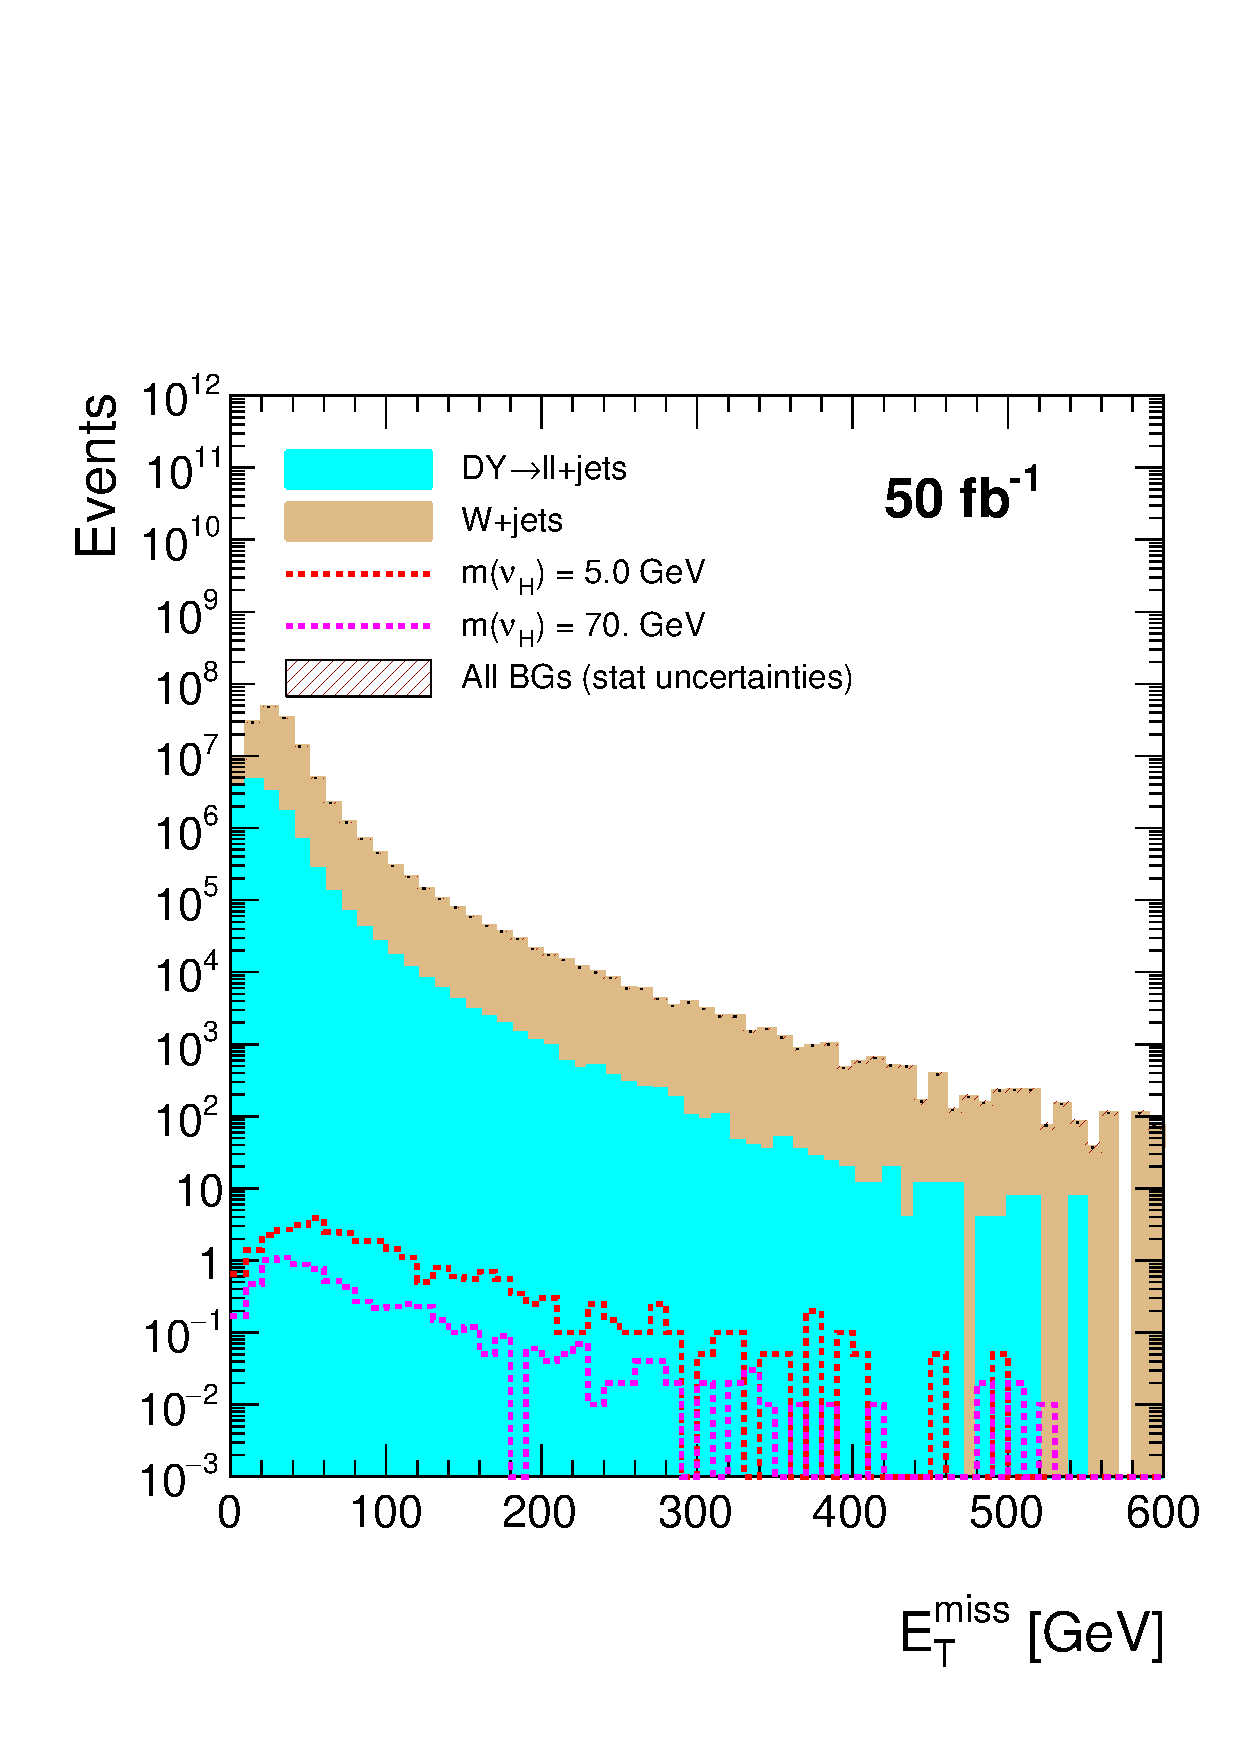
\includegraphics[width=0.8\textwidth]{./Capitulos/Analysis/AfterBJets/MET_MET_20} 
 \label{MET_bjets}
 \end{figure}
 
We studied the distribution of more variables in order to find possible cut values that can reduce the contribution of background. Figures \ref{HT_bjets}, \ref{diJetMass_bjets} and \ref{taupt_bjets} show the stacked plots of the variables $H_T$, di-jet mass and the tau $p_T$, respectively. These plots follow an analogous behavior as in the case of $\vec{E_T^{miss}}$: the number of background events is larger than of signal events and the background distribution is similar to the signal distribution. As a consequence, it is not possible to determine a set of variables that allow to reduce the contribution of background.
 
 \begin{figure}[h] 
 \centering
 \caption{Stacked plot of $H_T$ after the preselection cuts and cuts on the number of jets, taus and b-jets.}
 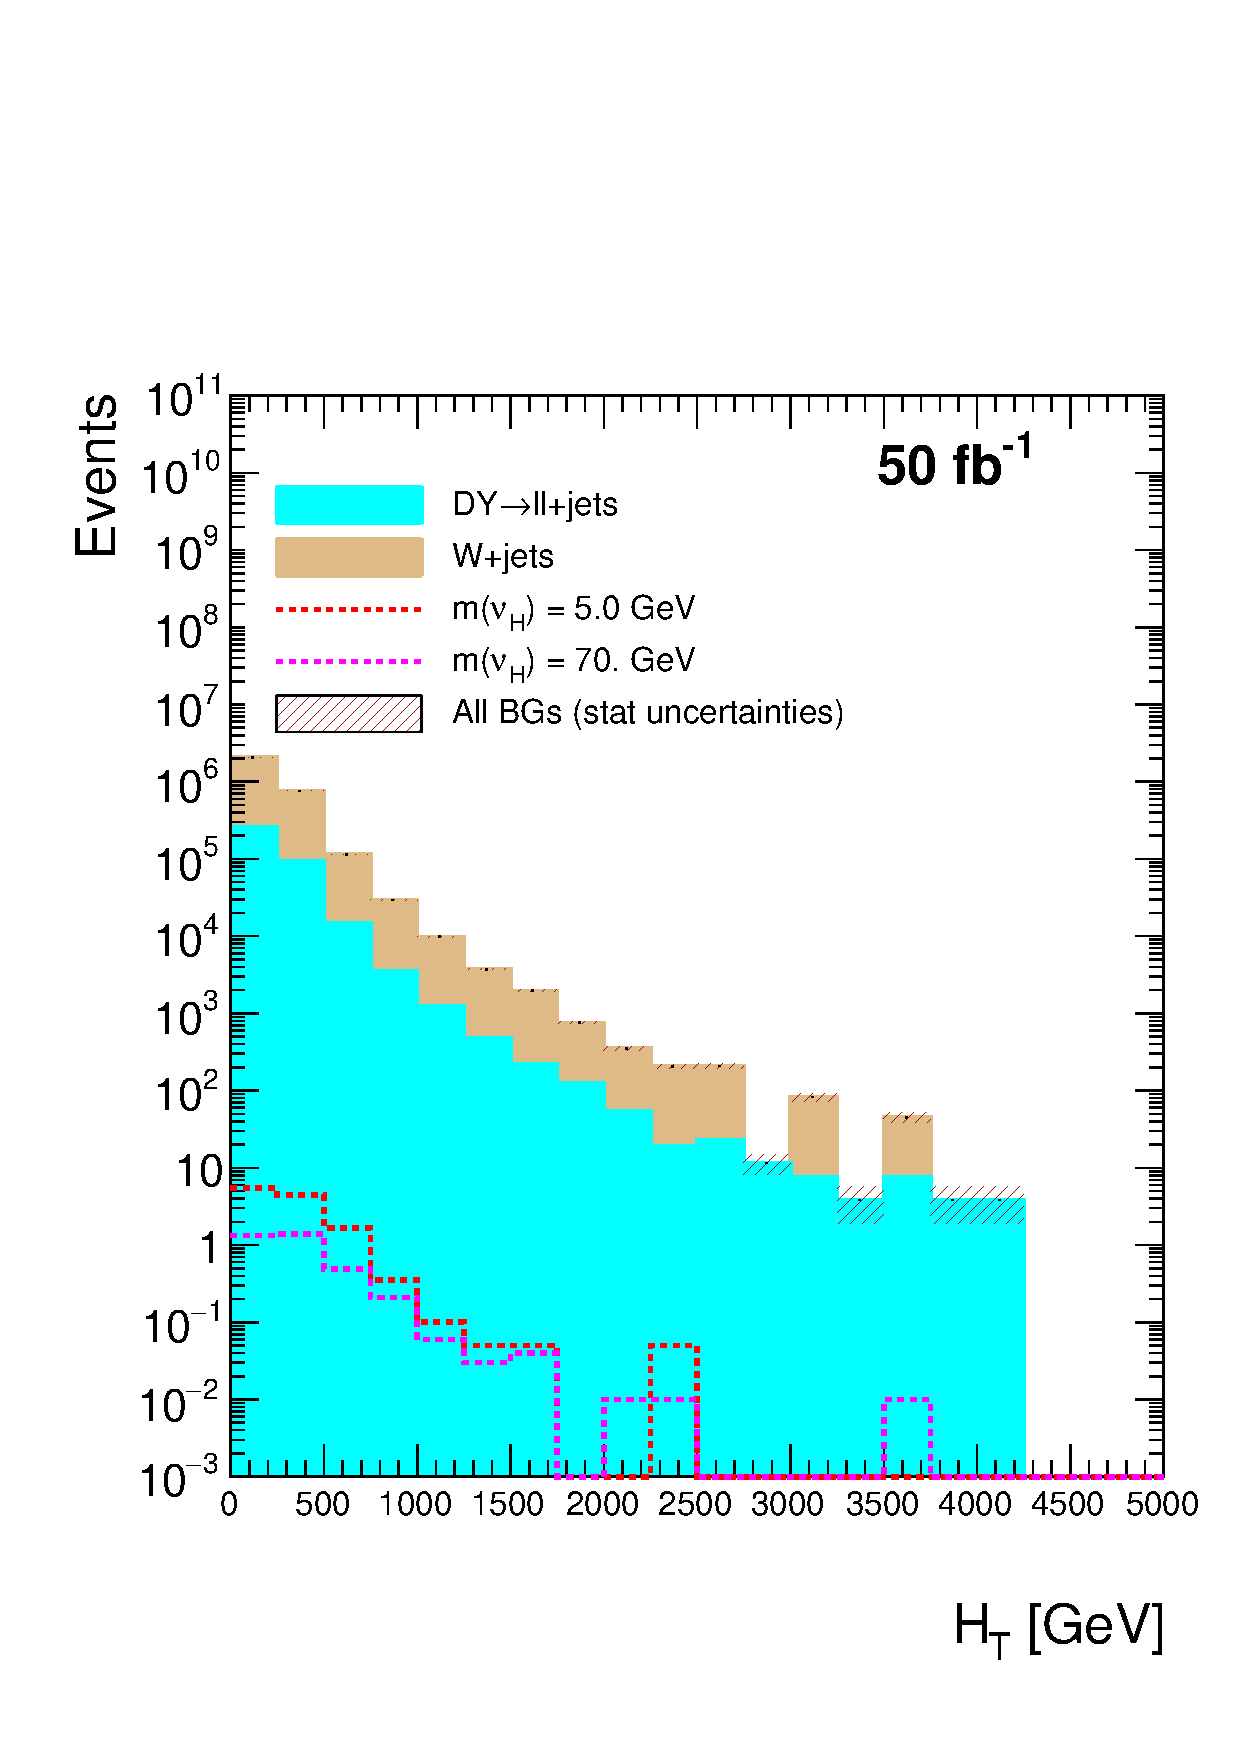
\includegraphics[width=0.7\textwidth]{./Capitulos/Analysis/AfterBJets/HT_MET_20} 
 \label{HT_bjets}
 \end{figure} 
 
  \begin{figure}[h] 
 \centering
 \caption{Stacked plot of di-jet mass after the preselection cuts and cuts on the number of jets, taus and b-jets.}
 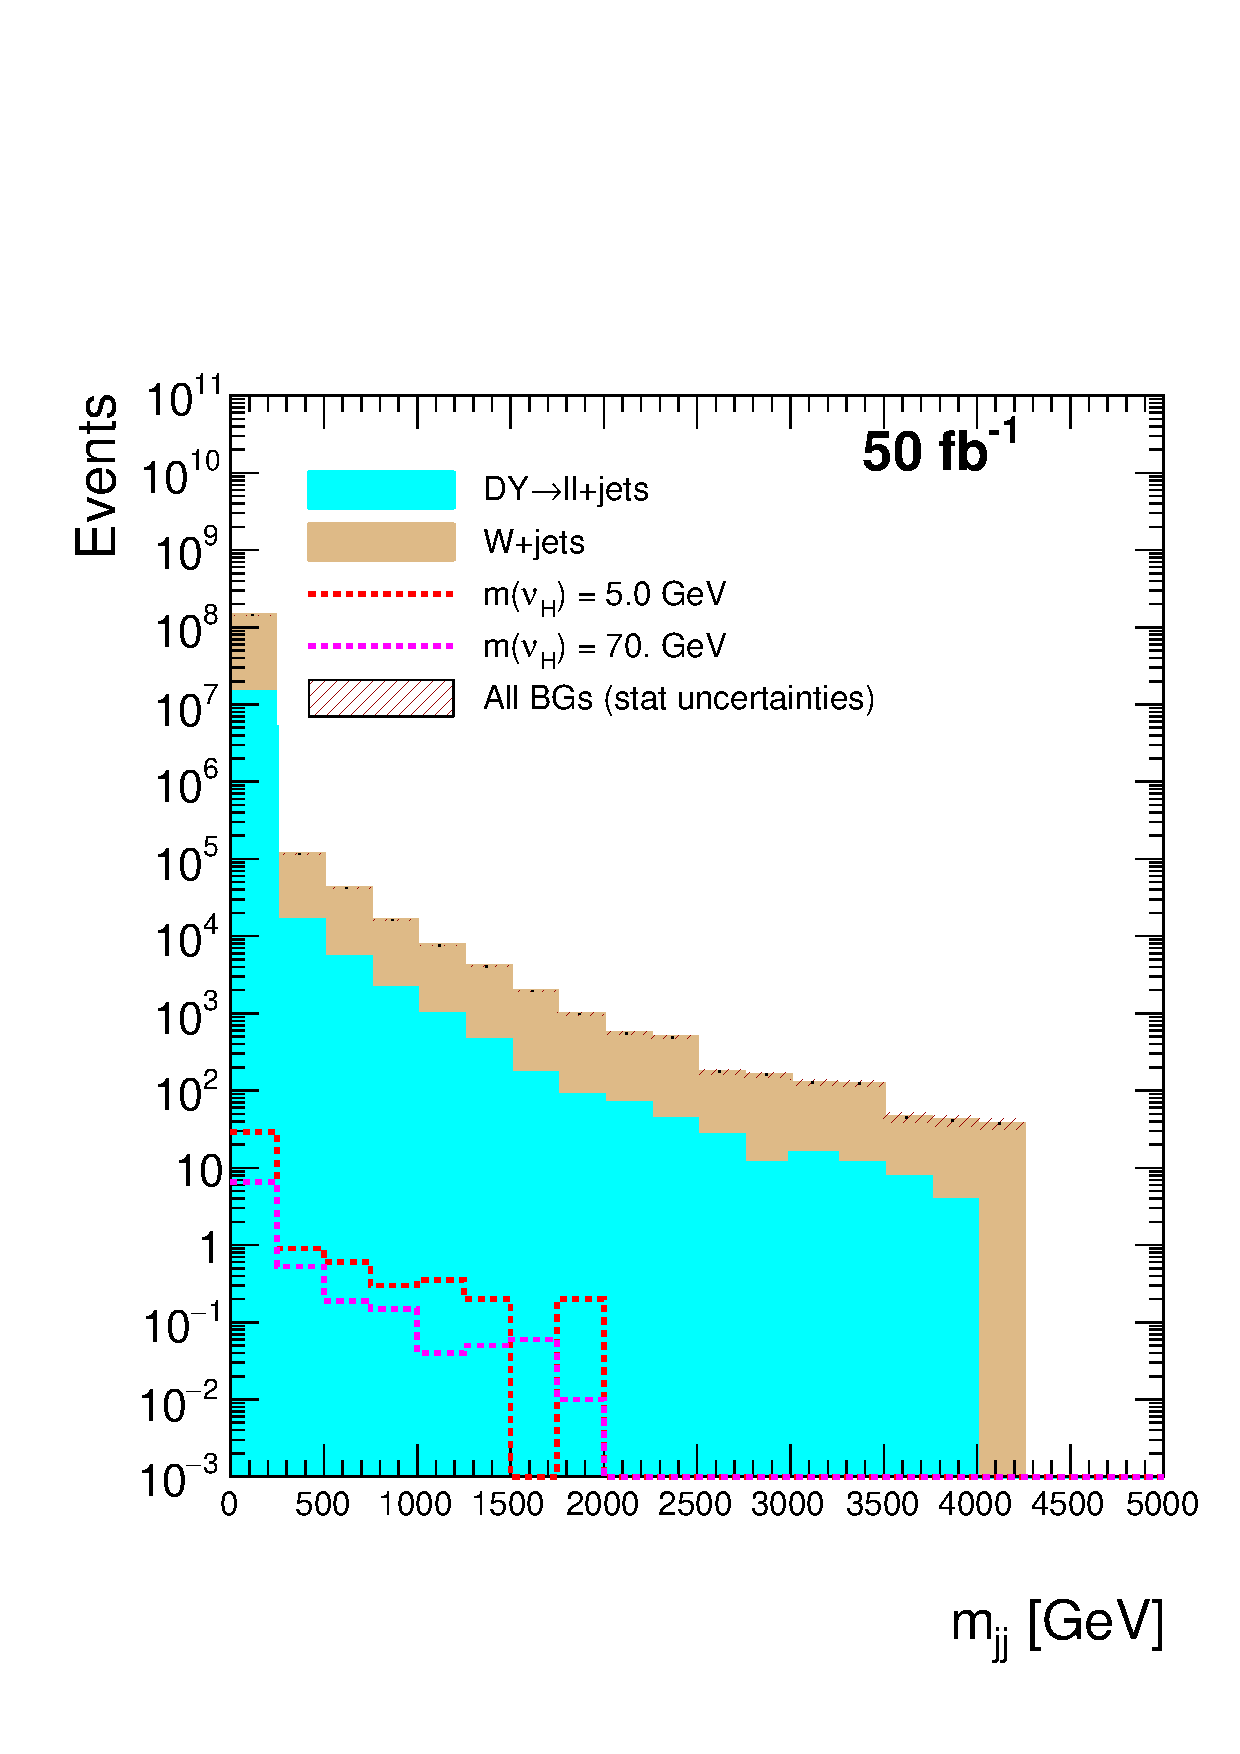
\includegraphics[width=0.7\textwidth]{./Capitulos/Analysis/AfterBJets/mjj_MET_20} 
 \label{diJetMass_bjets}
 \end{figure} 
 
  \begin{figure}[h] 
 \centering
 \caption{Stacked plot of $p_T(\tau)$ after the preselection cuts and cuts on the number of jets, taus and b-jets.}
 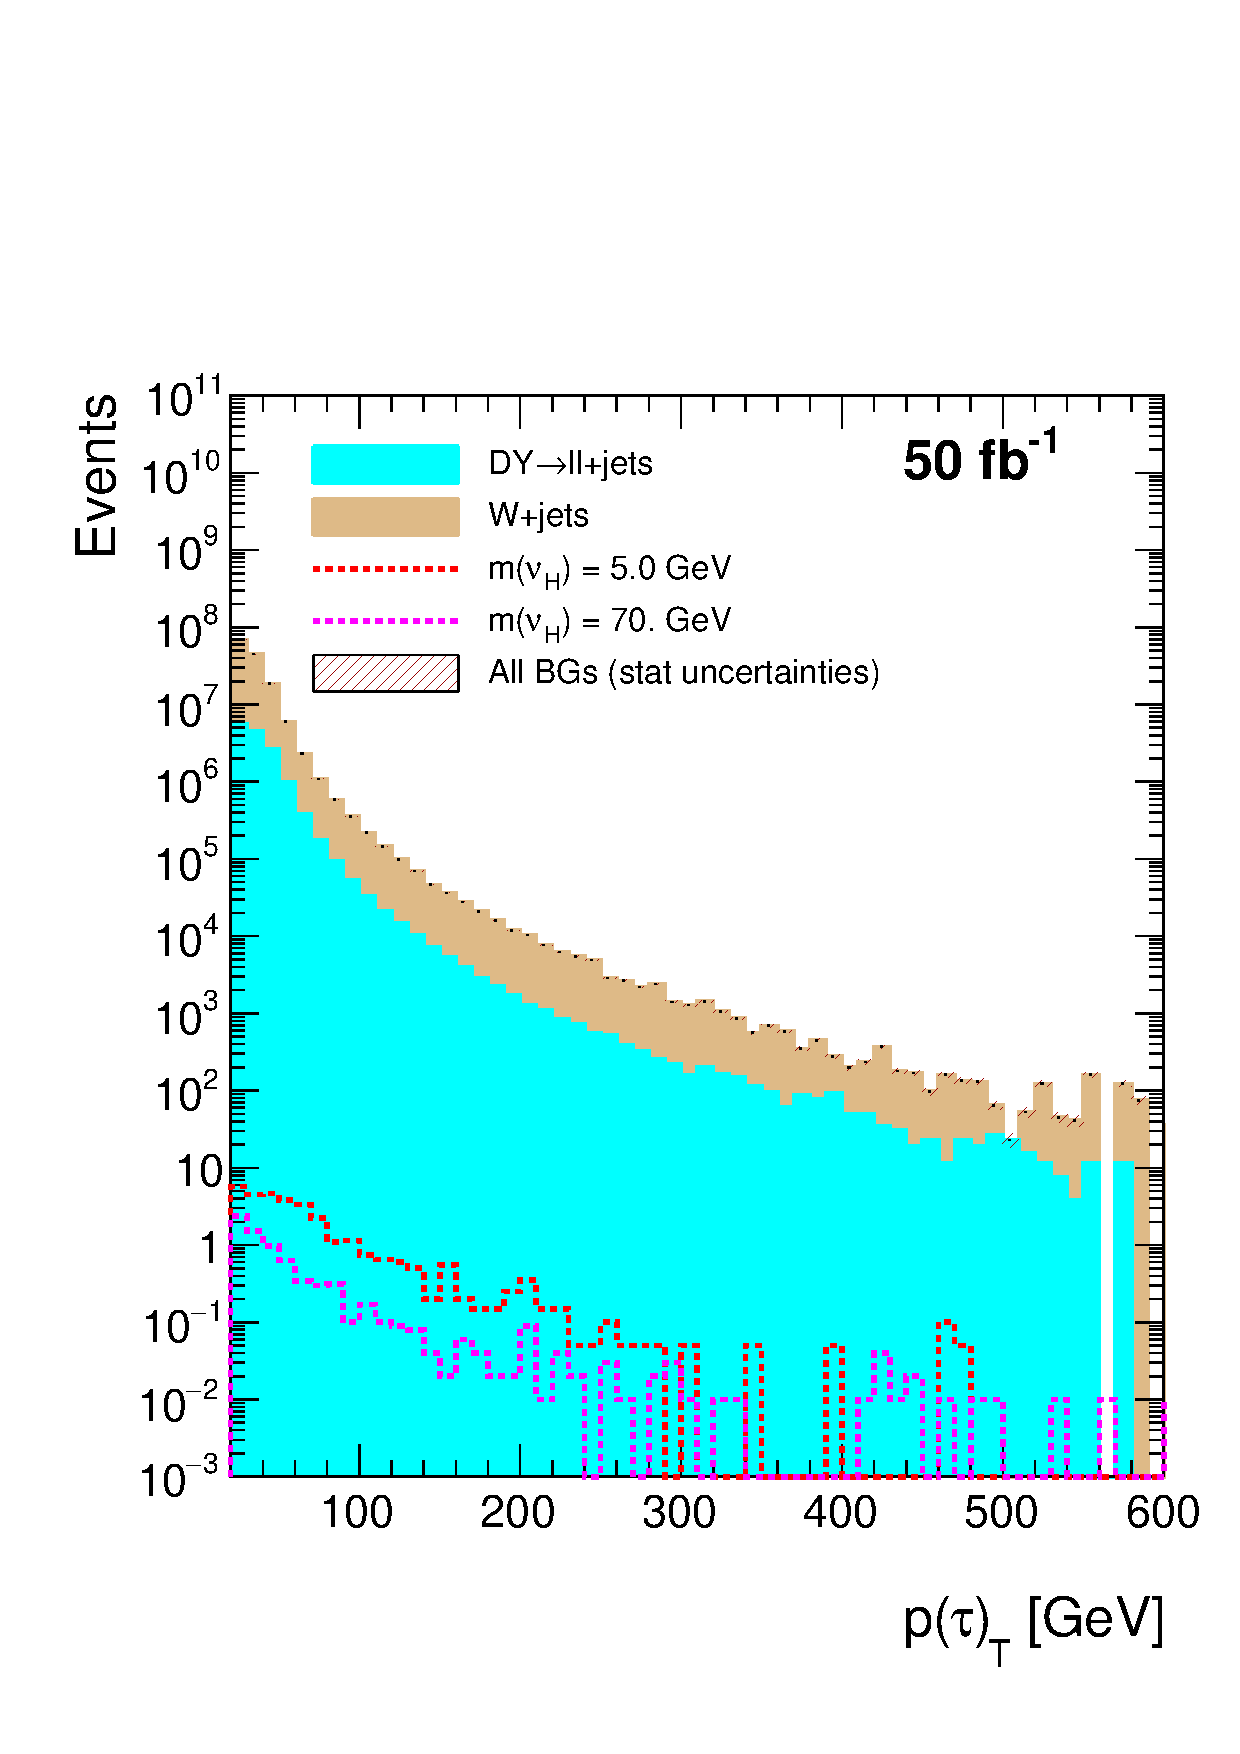
\includegraphics[width=0.7\textwidth]{./Capitulos/Analysis/AfterBJets/TauPt_MET_20} 
 \label{taupt_bjets}
 \end{figure} 
 
 Then, all the cuts mentioned in the Chapter \ref{Event_selection_criteria_chapter} are imposed. 
 These cuts include the cuts which take into account the topology of VBF processes. Figures \ref{HT_VBF}, \ref{diJetMass_VBF} and \ref{taupt_VBF} show the stacked plots of the $H_T$, di-jet mass and tau $p_T$ variables after all cuts, respectively. It can be seen that the quantity of background events reduces drastically, but it is still larger than the number of signal events. Moreover, the amount of signal events after imposing all cuts is minimal. Thus, it was not achievable to find a set of cuts that could reduce the background contribution in order to distinguish our signal of interest.
  
 
 \begin{figure}[h] 
 \centering
 \caption{Stacked plot of $H_T$ after the all the cuts were imposed.}
 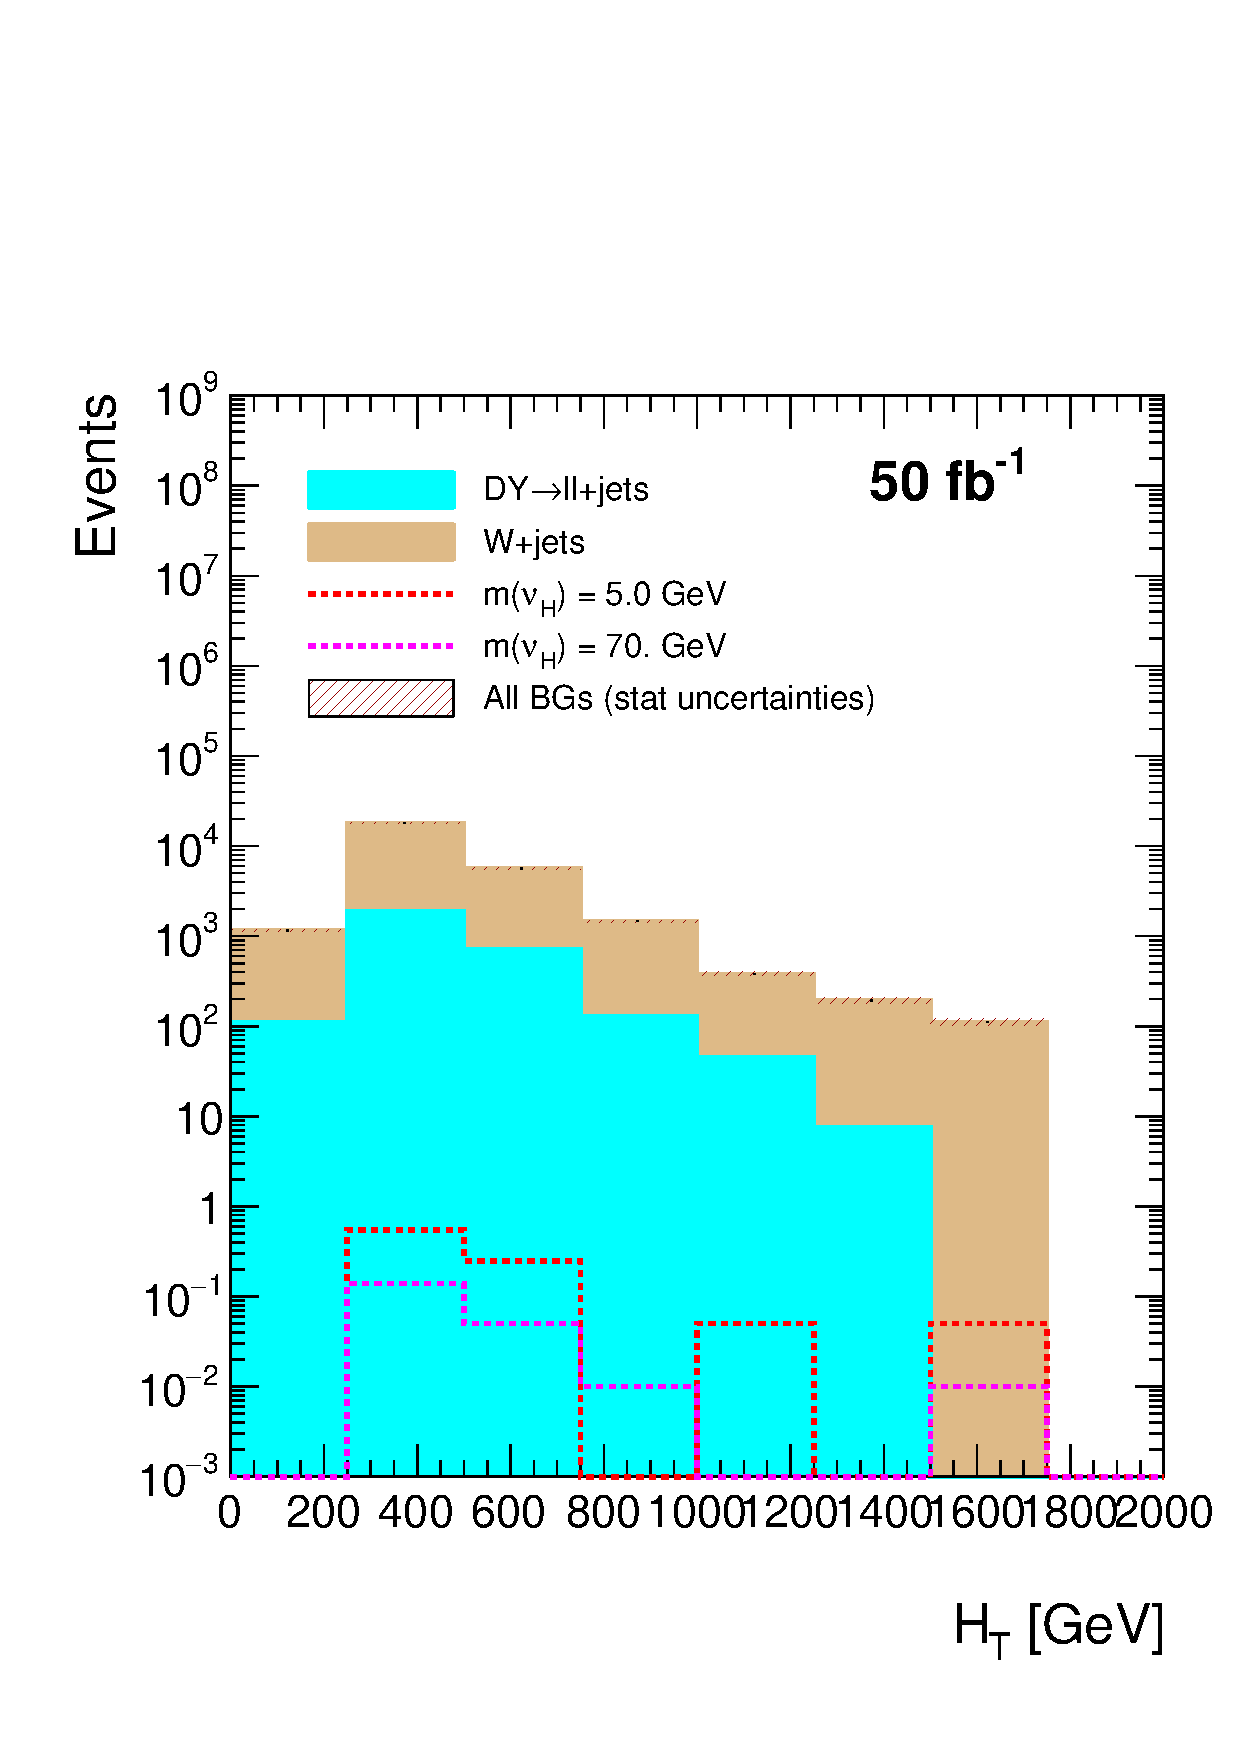
\includegraphics[width=0.7\textwidth]{./Capitulos/Analysis/AfterVBFCUTS/HT_MET_20} 
 \label{HT_VBF}
 \end{figure} 
 
  \begin{figure}[h] 
 \centering
 \caption{Stacked plot of di-jet mass after the all the cuts were imposed.}
 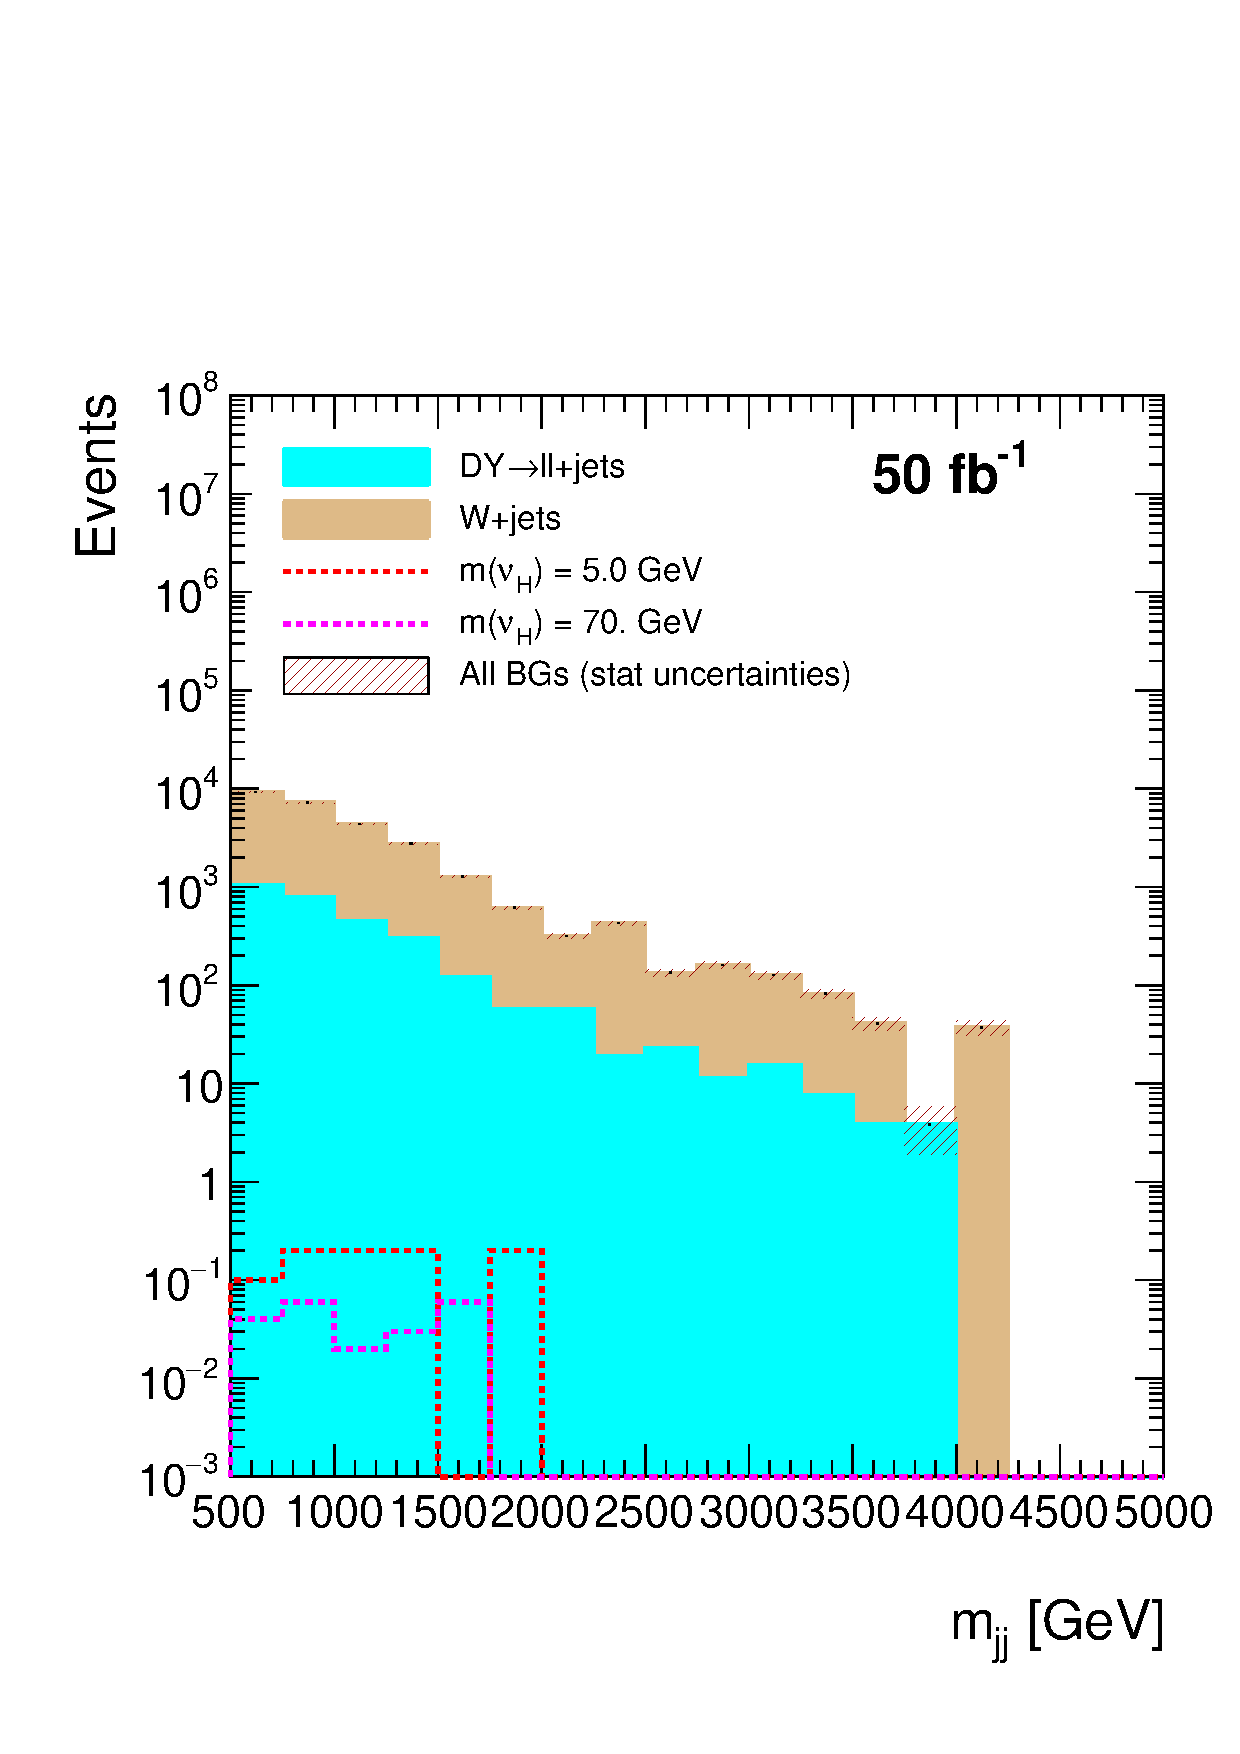
\includegraphics[width=0.7\textwidth]{./Capitulos/Analysis/AfterVBFCUTS/mjj_MET_20} 
 \label{diJetMass_VBF}
 \end{figure} 
 
  \begin{figure}[h] 
 \centering
 \caption{Stacked plot of $p_T(\tau)$ after the all the cuts were imposed.}
 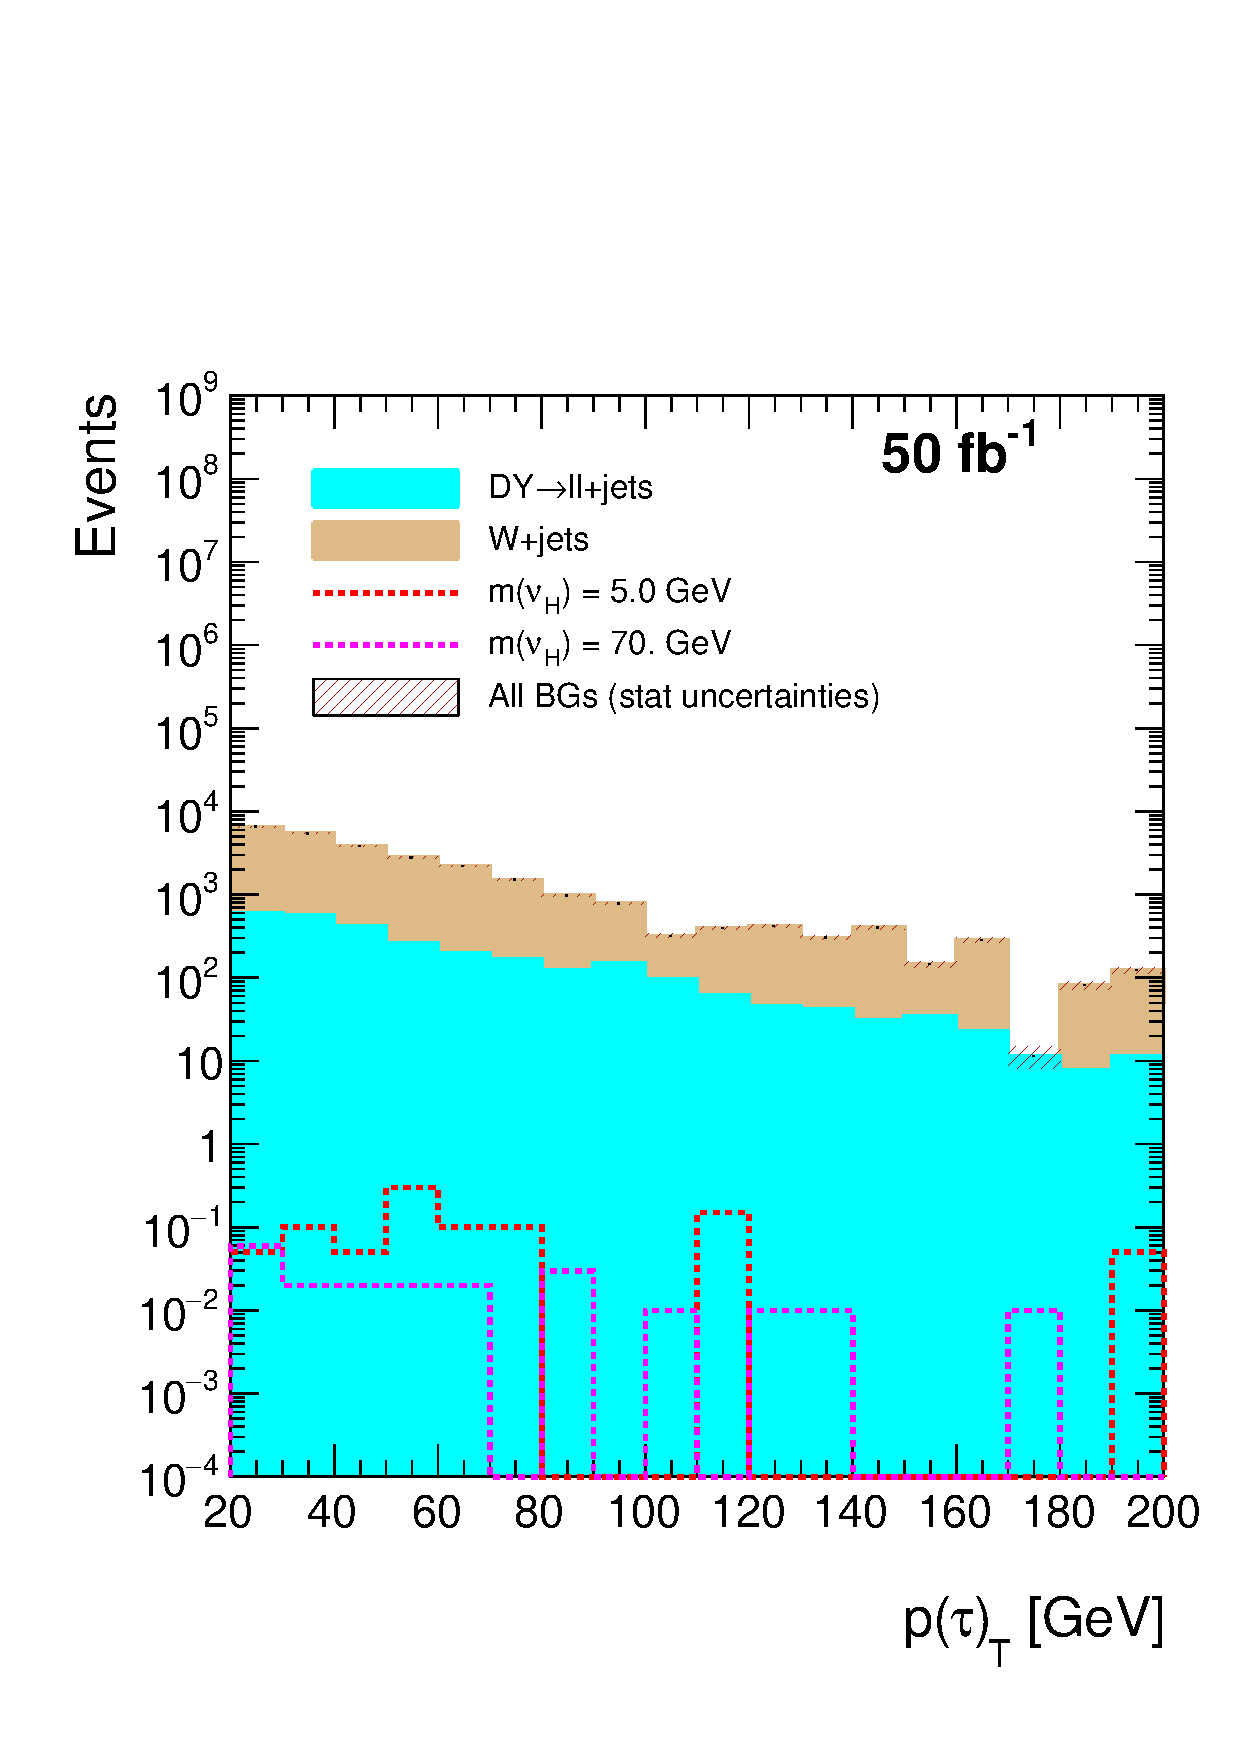
\includegraphics[width=0.7\textwidth]{./Capitulos/Analysis/AfterVBFCUTS/TauPt_MET20} 
 \label{taupt_VBF}
 \end{figure}  

One fact that can explain the reason why VBF cuts do not allow to reduce significantly the number of background events compared to the signal, is that the mass values of the Higgs boson and the Z boson are similar. Since this mass difference is almost just 30 GeV, the production mechanism of a Higgs boson is identical to the Z gamma production mechanism. Thus, the characteristics of the VBF jets in both events are similar and it is difficult to distinguish both VBF topologies. In the case that the heavy neutrinos are produced by the decay of a particle heavier that the Higgs boson, the heavier particle must be the result of an interaction between VBF jets with larger energy. Thus, in this case it would be expected that the detected VBF jets would be more energetic, which could allow to distinguish between both final states.

Since it was expected that the resulting tau in the signal had an associated track with a displaced vertex, some 2D plots were made using this variable. The value of the impact parameter for the tau was found by performing a minimization process on the distance between the tau and the tracks. 

First, we studied a plot on which the x axis 
represents $\vec{E_T^{miss}}$ and the y axis is the impact parameter ($d_{xy}$). This plot is shown in Figure \ref{ipt1_MET}. The first two plots at the left of this figure correspond to the signal events, one assuming a mass of the heavy neutrino of 5.0 GeV, and the other of 70.0 GeV. The range of the y axis for these plots is just from -1.0 to 1.0. The other two plots at the right of the figure correspond to the W+jets background and DY+jets background. These plots have a range in the y axis from -8.0 to 8.0. It can be seen that the impact parameter value of the signals is almost zero. This implies that it is not possible to make a cut on this variable to reduce the background as it was expected. Additionally, it is important to notice that in the case of the signals, the impact parameter only takes positive values which is not expected since the topology of the events should be symmetrical. 
 
 \begin{figure}[h] 
 \centering
 \caption{2D plot: $E_T^{miss}$ vs $d_{xy}$}
 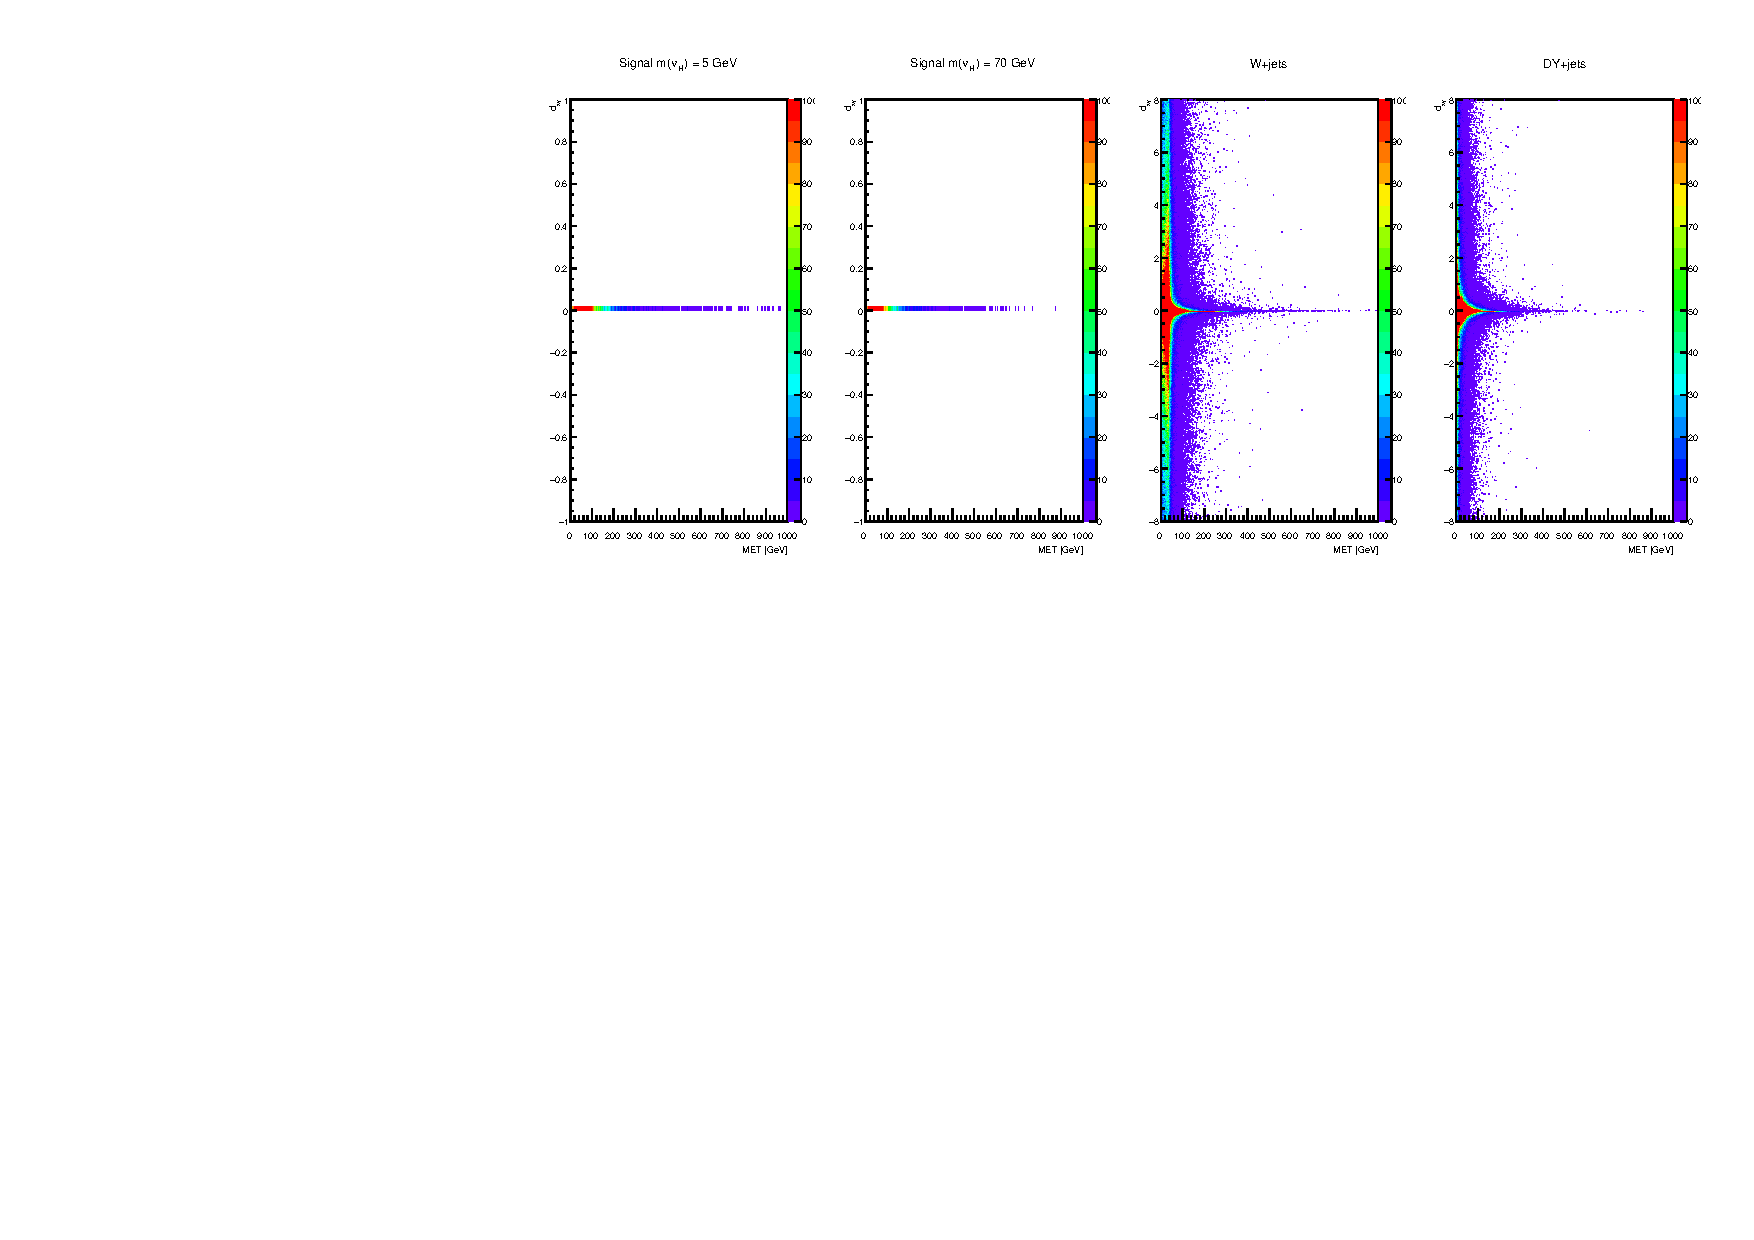
\includegraphics[width=1.15\textwidth]{./Capitulos/Analysis/c1} 
 \label{ipt1_MET}
 \end{figure}
 
Other 2D plots studied are shown in Figure \ref{ipt1_pt}. In these plots the x axis represents the tau transverse momentum and the y axis represents the absolute value of the impact parameter. In the signal plots, the y axis has a range between -0.1 to 0.4; while in the background plots it has a range between 0 and 8. Unfortunately, it is not possible to determine a cut value on any of these variables.
 
 \begin{figure}[h] 
 \centering
 \caption{2D plot: $p_T(\tau)$ vs $|d_{xy}|$}
 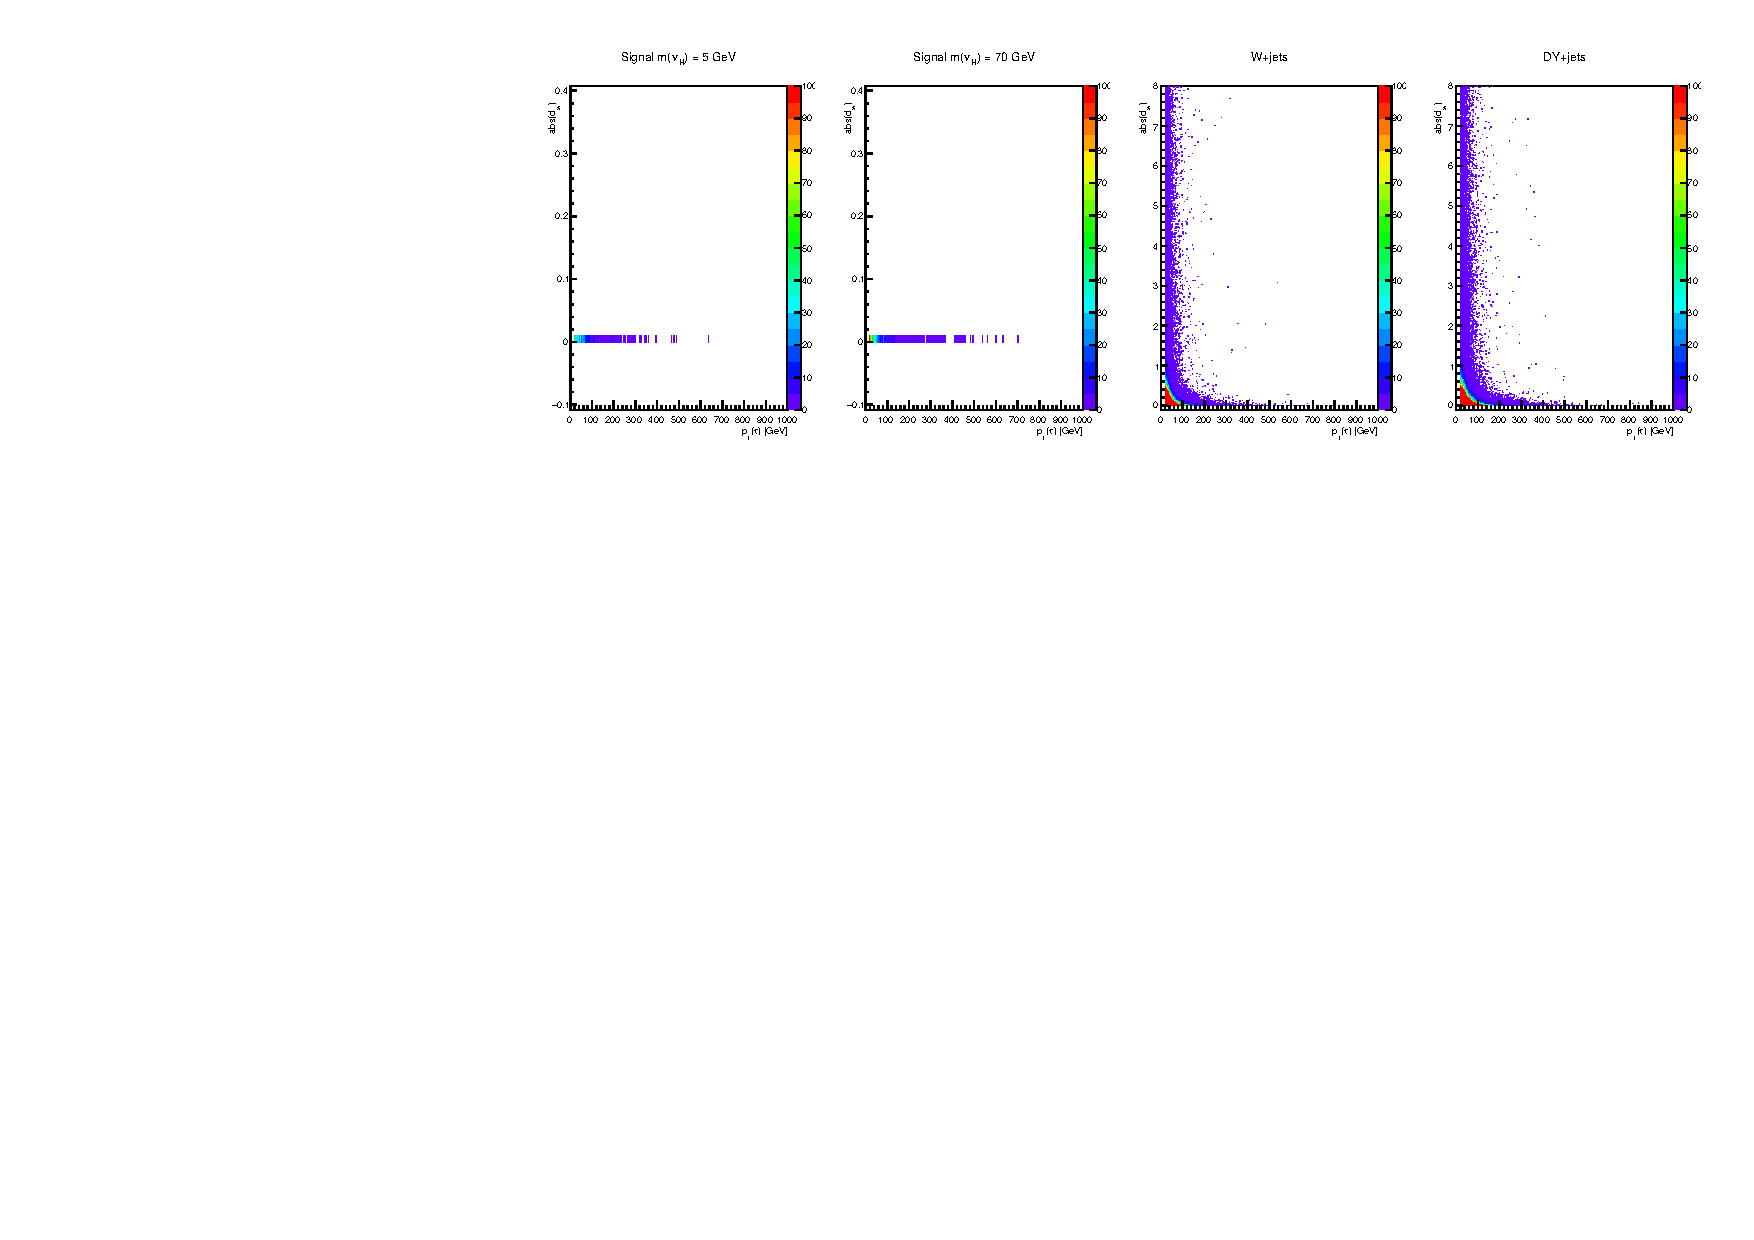
\includegraphics[width=1.15\textwidth]{./Capitulos/Analysis/ipt1_pt} 
 \label{ipt1_pt}
 \end{figure}
 
%EXPLICAR BIEN RECONSTRUCCION VERTICES Y MEJORAR GRAFICA 
 
Thus, we obtained that the signals of interest present a very low impact parameter value, while it was expected the opposite. Next, possible reasons that can explain the difference between our results and what was expected are discussed. In the first place, the quantity of signal events simulated is much smaller than the number of background events. Both simulated signals consisted of 10000 events, while the W+jets and DY+jets background samples consisted of millions of events. Thus, we had a small statistical sample and it may be necessary to generate more signal events to make the study. On the other hand, it seemed that there was a problem in the generation of the signals because their impact parameter values were only positive values. The former is not expected because there is no reason to believe that the impact parameter would have an asymmetric distribution. If this problem is solved, a cut on the impact parameter value would significantly reduce the amount of background.

%\thispagestyle{empty}
\chapter{Conclusions} 
\label{Conclusion_chapter}

The objetive of this work was to perfom a phenomenological analysis to determine a study that could reduce the backgrounds of our signal of interest under it. In order to do this, we started in Chapter \ref{State_Art_chapter} by making a brief summary of the SM and of what it states for neutrinos. Then, we studied the Majorana idea of writing the right-handed field in terms of the left-handed field. The former leads to the description of a Majorana mass term and the definition of a Majorana particle. Then, it is analized the Seesaw mechanism and the explanations it has for the mass of neutrinos are discussed. After, in Chapter \ref{Important_concepts_chapter} the relevant concepts and kinematical variables for this analysis were defined and explained.

In the chapter \ref{CMS_chapter} the different parts of the CMS detector are described with the explanation of how they work and their characteristics. The CMS detector was explained with detail because in this analysis we considered events generated at this detector. Next, in chapter \ref{Model_chapter} the topology of the signals are explained: it is expected that the product tau has a displaced vertex, the presence of high energetic jets related to the VBF process, among other characteristics. The backgrounds of these signals were also explained with their final state characteristics. After, in the Chapter \ref{Methodology_chapter} the computational tools that were used in this analysis are described. It was mentioned each software and their specific task on the simulation of the signal or analysis of the data.  

Then, the preselection criteria and the different cuts that were applied in this analysis were stated and explained in the Chapter \ref{Event_selection_criteria_chapter}. The following Chapter \ref{Analysis_chapter} showed the analysis that was perfomed to study the signal and its background. It was showed that it was not possible to find optimal cuts in order to reduce the amount of background under the magnitude of the signal. The former was because, as it was shown, the kinematical and topological distributions of the signals and backgrounds were very similar.
Additionally, the obtained the values of the impact parameter for the signals were unexpected, because they were very low and it was expected they had a large impact parameter value. The former can be a consequence that the size of the signal sample was small and that Delphes does not correctly reconstruct the secondaray vertices.



%\thispagestyle{empty}

%----------------------------------------------------------------------------------------
%	APÉNDICES
%----------------------------------------------------------------------------------------

%\addtocontents{toc}{\vspace{2em}} % Agrega espacios en la toc

%\appendix % Los siguientes capítulos son apéndices
\begin{appendices}
%  Incluye los apéndices en el folder de apéndices

%\chapter{Neutrinos and Seesaw Mechanism} \label{apendice_neutrinos}


\subsection{Dirac Mass}
In this Appendix we are going to perform with detail the calculations for neutrino physics which where described in the State of the Art chapter. 
We start here by studying the Dirac Mass wich was a term of the form:

\begin{equation}
 m \overline{\psi} \psi = m \overline{(\psi_L + \psi_R)} (\psi_L + \psi_R) = m(\overline{\psi_L} \psi_L + \overline{\psi_L}\psi_R + \overline{\psi_R}\psi_L + \overline{\psi_R} \psi_R)
\end{equation}

Lets study the term $\overline{\psi_L}\psi_L$ and using $P_R  P_L = 0$:

\begin{equation}
 \overline{\psi_L}\psi_L = \overline{\psi} {P}^{\dagger}_L P_L \psi = \overline{\psi}P_R  P_L \psi = 0
\end{equation}

Using an analogous reasoning we can find $\overline{\psi_R}\psi_R = 0$, too. Finally, we obtain the expresion:

\begin{equation}
  m \overline{\psi} \psi = m (\overline{\psi_L} \psi_R + \overline{\psi_R}\psi_L)
\end{equation}

\subsection{Majorana Mass}

The expresion we had for the Dirac Lagrangian was: 

\begin{align}
  %\phantom{i = j = k}
  &\begin{aligned}
    \mathllap{L} &= \overline{\psi} \left( i \gamma ^\mu \partial_{\mu} - m \right) \psi \\
    \mathllap{}  &= (\overline{\psi_L} + \overline{\psi_R})( i \gamma ^\mu \partial_{\mu} - m)(\psi_L + \psi_R) \\
    \mathllap{}  &= i \overline{\psi_L} \gamma ^\mu \partial_{\mu} \psi_L + i \overline{\psi_L} \gamma ^\mu   \partial_{\mu} \psi_R - m \overline{\psi_L} \psi_L - m \overline{\psi_L} \psi_R \\
  &\qquad + i \overline{\psi_R} \gamma ^\mu \partial_{\mu} \psi_L + i \overline{\psi_R} \gamma^{\mu} \partial_{\mu} \psi_R - m \overline{\psi_R} \psi_L - m \overline{\psi_R} \psi_R \\
  \end{aligned}\\
\end{align}

We already proved that $\overline{\psi_L}\psi_L = \overline{\psi_R}\psi_R = 0$. Now we study the second term in the latest equation, which has a term of the form:
\begin{align}
  &\begin{aligned}
     \mathllap{P_R\gamma^\mu}  &= \frac{1}{2} (1 + \gamma^5)\gamma^\mu = \frac{1}{2} (\gamma^\mu + \gamma^5 \gamma^\mu) \\        
     \mathllap{}            &= \frac{1}{2} (\gamma^\mu - \gamma^\mu \gamma^5) & \text{Since $\{\gamma^5,\gamma^\mu\} = \gamma^5\gamma^\mu + \gamma^\mu \gamma^5 = 0$} \\
     \mathllap{}            &= \frac{1}{2} \gamma^\mu (1 - \gamma^5) = \gamma^\mu P_L 
  &\end{aligned}
\end{align}

Using what we have found in the last expression, we get for the second term:
\begin{align}
  &\begin{aligned}
     \mathllap{i\overline{\psi_L}\gamma^\mu \partial_\mu \psi_R}  &=  i \overline{\psi}P_R \gamma^\mu \partial_\mu P_R \psi\\        
     \mathllap{}            &=  i \overline{\psi}\gamma^\mu P_L \partial_\mu P_R\psi \\
     \mathllap{}            &=  i \overline{\psi}\gamma^\mu \partial_\mu P_L P_R \psi && \text{Since $P_L$ is a constant operator}\\
     \mathllap{}            &=  0
  &\end{aligned}
\end{align}

Following a similar calculus we get: $i\overline{\psi_R}\gamma^\mu \partial_\mu \psi_L$ = 0. Our next step is to find the two coupled Dirac equations using the Euler-Lagrange equation. We obtained for the Lagrangian:

\begin{equation}
L = i \overline{\psi_R} \gamma^\mu \partial_\mu \psi_R + i \overline{\psi_L}\gamma^\mu \psi_L -m\overline{\psi_R}\psi_L - m \psi_L\psi_R
\end{equation}

Replacing in the Euler-Lagrange equation we get for both states:
\begin{align}
  &\begin{aligned}
     \mathllap{\frac{\partial L}{\partial(\partial \overline{\psi_R})}}  &=  \frac{\partial L}{\partial \overline{\psi_R}} \ \ \rightarrow \ \ 0 = i \gamma^\mu \partial_\mu \psi_L -m \psi_R  \\        
     \mathllap{\frac{\partial L}{\partial(\partial \overline{\psi_L})}}  &=  \frac{\partial L}{\partial \overline{\psi_L}} \ \ \rightarrow \ \ 0 = i \gamma^\mu \partial_\mu \psi_R -m \psi_L\\ 
  &\end{aligned} \label{major start}
\end{align}

Now, we are going to find an expression for $\psi_R$ in terms of $\psi_L$. We take the hermitian conjugate of the equation $\ref{major start}$:

\begin{align}
  &\begin{aligned}
     \mathllap{(i \gamma^\mu \partial_\mu \psi_R)^\dagger}  &= m\psi_L^\dagger 
  &\end{aligned}
\end{align}





 
\thispagestyle{empty}
\chapter{Neutrinos and Seesaw Mechanism} 
\label{apendice_neutrinos}

First of all we are going to start by defining some fundamental concepts: helicity, chirality and projection operators. The helicity of a particle is defined as the projection of its spin onto the direction of its motion. It is said that a particle is right-handed when its spin is in the same direction as its motion and it is said a particle is left-handed when its spin is opposite in the opposite direction of its motion. In the case of massless particles the concept of chirality and helicity is equivalent. The chirality for a Dirac fermion is defined through the operator $\gamma^5$ with eigenvalues $\pm 1$. Thus a Dirac field can be projected into its left or right component by acting the operators $P_R$ and $P_L$ upon it. The right- and left-handed projection operators are defined as:
\begin{equation}
P_R = \frac{1 + \gamma^5}{2} \ \ \text{and } \ \ P_L = \frac{1 - \gamma^5}{2}
\end{equation}


\subsection{Dirac Mass}
In this Appendix, we are going to perform with detail the calculations for neutrino physics which were mentioned in the State of the Art Chapter. 
We start here by studying the Dirac Mass, which is a term of the form:

\begin{equation}
 m \overline{\psi} \psi = m \overline{(\psi_L + \psi_R)} (\psi_L + \psi_R) = m(\overline{\psi_L} \psi_L + \overline{\psi_L}\psi_R + \overline{\psi_R}\psi_L + \overline{\psi_R} \psi_R)
\end{equation}

Lets study the term $\overline{\psi_L}\psi_L$ and using $P_R  P_L = 0$:

\begin{equation}
 \overline{\psi_L}\psi_L = \overline{\psi} {P}^{\dagger}_L P_L \psi = \overline{\psi}P_R  P_L \psi = 0
\end{equation}

Using an analogous reasoning, we can find $\overline{\psi_R}\psi_R = 0$, too. Finally, we obtain the expresion:

\begin{equation}
  m \overline{\psi} \psi = m (\overline{\psi_L} \psi_R + \overline{\psi_R}\psi_L)
\end{equation}

\subsection{Majorana Mass}

The expression we had for the Dirac Lagrangian was: 
%REVISARRRRRRRRRRRRRRR
\begin{align}
  %\phantom{i = j = k}
  &\begin{aligned}
    \mathllap{L} &= \overline{\psi} \left( i \gamma ^\mu \partial_{\mu} - m \right) \psi \\
    \mathllap{}  &= (\overline{\psi_L} + \overline{\psi_R})( i \gamma ^\mu \partial_{\mu} - m)(\psi_L + \psi_R) \\
    \mathllap{}\label{Expresion_Dirac}  &= i \overline{\psi_L} \gamma ^\mu \partial_{\mu} \psi_L + i \overline{\psi_L} \gamma ^\mu   \partial_{\mu} \psi_R - m \overline{\psi_L} \psi_L - m \overline{\psi_L} \psi_R \\
  &\qquad + i \overline{\psi_R} \gamma ^\mu \partial_{\mu} \psi_L + i \overline{\psi_R} \gamma^{\mu} \partial_{\mu} \psi_R - m \overline{\psi_R} \psi_L - m \overline{\psi_R} \psi_R \\
  \end{aligned}
\end{align}

We already proved that $\overline{\psi_L}\psi_L = \overline{\psi_R}\psi_R = 0$. Now we are going to study the second term in the Equation \ref{Expresion_Dirac}, which has a term of the form:

\begin{align}
  &\begin{aligned}
     \mathllap{P_R\gamma^\mu}  &= \frac{1}{2} (1 + \gamma^5)\gamma^\mu = \frac{1}{2} (\gamma^\mu + \gamma^5 \gamma^\mu) \\        
     \mathllap{}            &= \frac{1}{2} (\gamma^\mu - \gamma^\mu \gamma^5) & \text{Since $\{\gamma^5,\gamma^\mu\} = \gamma^5\gamma^\mu + \gamma^\mu \gamma^5 = 0$} \\
     \mathllap{}            &= \frac{1}{2} \gamma^\mu (1 - \gamma^5) = \gamma^\mu P_L 
  &\end{aligned}
\end{align}

Using what we have found in the last expression, we get for the second term:
\begin{align}
  &\begin{aligned}
     \mathllap{i\overline{\psi_L}\gamma^\mu \partial_\mu \psi_R}  &=  i \overline{\psi}P_R \gamma^\mu \partial_\mu P_R \psi\\        
     \mathllap{}            &=  i \overline{\psi}\gamma^\mu P_L \partial_\mu P_R\psi \\
     \mathllap{}            &=  i \overline{\psi}\gamma^\mu \partial_\mu P_L P_R \psi && \text{Since $P_L$ is a constant operator}\\
     \mathllap{}            &=  0
  &\end{aligned}
\end{align}

Following a similar calculation we get: $i\overline{\psi_R}\gamma^\mu \partial_\mu \psi_L$ = 0. Our next step is to find the two coupled Dirac equations using the Euler-Lagrange equation. We 
obtained for the Lagrangian:   

\begin{equation}
L = i \overline{\psi_R} \gamma^\mu \partial_\mu \psi_R + i \overline{\psi_L}\gamma^\mu \psi_L -m\overline{\psi_R}\psi_L - m \psi_L\psi_R
\end{equation}

Replacing in the Euler-Lagrange equation, we get for both states:
\begin{align}
  &\begin{aligned}\label{major start}
     \mathllap{\frac{\partial L}{\partial(\partial \overline{\psi_R})}}  &=  \frac{\partial L}{\partial \overline{\psi_R}} \ \ \rightarrow \ \ 0 = i \gamma^\mu \partial_\mu \psi_L -m \psi_R  \\        
     \mathllap{\frac{\partial L}{\partial(\partial \overline{\psi_L})}}  &=  \frac{\partial L}{\partial \overline{\psi_L}} \ \ \rightarrow \ \ 0 = i \gamma^\mu \partial_\mu \psi_R -m \psi_L\\ 
  &\end{aligned} 
\end{align}

Now, we are going to find an expression for $\psi_R$ in terms of $\psi_L$. First, we take the hermitian conjugate of the bottom equation in \ref{major start}:

\begin{align}
  &\begin{aligned}
     \mathllap{i \gamma^\mu \partial_\mu \psi_R} &= m\psi_L\\        
     \mathllap{(i \gamma^\mu \partial_\mu \psi_R)^\dagger} &= m\psi_L^\dagger  & \text{Taking the hermitian conjugate} \\
     \mathllap{-i \partial_\mu \psi_R^\dagger \gamma^{\mu \dagger}} &= m \psi_L^\dagger \\
     \mathllap{-i \partial_\mu \psi_R^\dagger \gamma^{\mu \dagger}\gamma^0} &= m \psi_L^\dagger \gamma^0  &\text{Multiplying on the right by $\gamma^0$}\\
     \mathllap{-i \partial_\mu \psi_R^\dagger \gamma^0 \gamma^\mu} &= m \psi_L^\dagger \gamma^0  &\text{Using $\gamma^{\mu \dagger}\gamma^0 = \gamma^0 \gamma^\mu$ }\\    %\leftarrow \gamma^0(\gamma^0 \gamma^{\mu \dagger}\gamma^0) = \gamma^0(\gamma^\mu$) }\\
     \mathllap{-i \partial_\mu \overline{\psi_R}\gamma^\mu} &= m \overline{\psi_L} &\text{We have $\overline{\psi} = \psi^{\dagger}\gamma^0$}\\
     \mathllap{-i (\partial_\mu \overline{\psi_R}\gamma^\mu)^\intercal} &= m \overline{\psi_L}^\intercal &\text{Taking the transpose}\\
     \mathllap{-i \gamma^{\mu \intercal} \partial_\mu \overline{\psi_R}^\intercal} &= m \overline{\psi_L}^\intercal \\
     \mathllap{-i (-C^{-1}\gamma^\mu C) \partial_\mu \overline{\psi_R}^\intercal} &= m \overline{\psi_L}^\intercal &\text{Using $\gamma^{\mu \intercal}= -C^{-1}\gamma^\mu C$}\\
     \mathllap{i \gamma^\mu \partial_\mu C \overline{\psi_R}^\intercal} &= m C \overline{\psi_L}^\intercal &\text{Multiplying on the left by C}\\
  &\end{aligned}
\end{align}

As we saw previously, for the last equation to have a similar structure as the top equation of \ref{major start}, the right-handed component of $\psi$ must be:

\begin{equation}
 \psi_R = C \overline{\psi_L}^\intercal
\end{equation}

Now, we need to prove that $C \overline{\psi_L}^\intercal$ is actually right-handed. To do this we apply the left-handed chiral projection operator $P_L$ on this state and
the result must be zero.

\begin{align}
  &\begin{aligned}
     \mathllap{P_L \left( C \overline{\psi_L}^\intercal \right)} &= C P_L^\intercal \overline{\psi_L}^\intercal &\text{Property of C: $P_LC = C P_L^\intercal$}\\        
     \mathllap{} &= C \left( \overline{\psi_L}P_L \right)^\intercal  
  &\end{aligned}
\end{align}

Now, let us examine the term $\overline{\psi_L}P_L$:
 
%REVISARRRRRRRRRRRRRRR TERMINO

\begin{align}
  &\begin{aligned}
    \mathllap{\overline{\psi_L}P_L} &= (P_L \psi)^\dagger \gamma_0 P_L = \psi^\dagger P_L \gamma_0 P_L\\
    \mathllap{} &= \psi^\dagger \gamma^0 P_R P_L = 0
    &\end{aligned}
\end{align}

Hence $C \overline{\psi_L}^\intercal$ is in fact a right-handed quiral state. 
\\

\subsection{Seesaw Mechanism}

Now, let us find the neutrino mass values by diagonalizing the matrix M:

\begin{equation}
M = 
  \begin{pmatrix}
  m_L & m_D \\
  m_D & m_R  
  \end{pmatrix}
\end{equation}

In order to find the mass eigenvalues we need to solve the equation:
\begin{equation}
\left| M - I \lambda \right|  = \left| \begin{pmatrix}
  m_L - \lambda & m_D \\
  m_D & m_R - \lambda 
  \end{pmatrix} \right| = 0
\end{equation}

We obtain a quadratic equation of the form: 

\begin{equation}
\lambda ^2 - (m_L + m_R) \lambda + (m_L m_R - m_D^2) = 0
\end{equation}

Using the quadratic equation to find the values of $\lambda$, we get:

\begin{align}
  &\begin{aligned}
     \mathllap{m_{1,2}} &= \frac{(m_L + m_R) \pm \sqrt{(m_L + m_R)^2 - 4 (m_L m_R - m_D^2)}}{2} \\
     \mathllap{}        &= \frac{(m_L + m_R) \pm \sqrt{(m_L - m_R)^2 - 4 m_D^2)}}{2}
  &\end{aligned}
\end{align}

Now, setting $m_L= 0$ and assuming $m_R >> m_D$, we obtain the following mass eigenstates. For the 
neutrino field $\nu_1$ the mass is given by Equation \ref{mass1}, and for the neutrino field $\nu_2$ the mass is give by the Equation \ref{mass2}.

\begin{equation}
m_1 = \frac{m_D^2}{m_R}
\label{mass1}
\end{equation}

\begin{equation}
m_2 = m_R \left( 1 + \frac{m_D^2}{m_R^2} \right) \approx m_R
\label{mass2}
\end{equation}
%\chapter{Charge Conjugation Operator} \label{appendix_charge_conjugation}
%\include{Apendices/AppendixC}
\end{appendices}

\addtocontents{toc}{\vspace{2em}} % Agrega espacio en la toc


%----------------------------------------------------------------------------------------
%	BIBLIOGRAFÍA
%----------------------------------------------------------------------------------------
%\backmatter
%\nocite{*}
%\bibliographystyle{plain}
%\bibliography{bibliografía.bib} %Aquí ponen el nombre del archivo .bib


\begin{thebibliography}{10}

\bibitem{Neutrino experiment 1 mass} Gonzalez-Garcia, M., Maltoni, M., \& Schwetz, T. (2016). Global analyses of neutrino oscillation experiments. Nuclear Physics B, 908, 199-217. http://dx.doi.org/10.1016/j.nuclphysb.2016.02.0331

\bibitem{Neutrino experiment 2 mass} Balantekin, A. \& Haxton, W. (2013). Neutrino oscillations. Progress In Particle And Nuclear Physics, 71, 150-161. http://dx.doi.org/10.1016/j.ppnp.2013.03.007   
 
\bibitem{Neutrino dark matter candidate 1} Bhupal, P.S., Mohapatra, R.N., and Zhang, Y. (2016). Heavy right-handed neutrino dark matter in left-right models. Retrieved from https://arxiv.org/abs/1610.05738     

\bibitem{Neutrino dark matter candidate 2} Bhupal, P.S., Mohapatra, R.N., and Zhang, Y. (2016). Naturally Stable Right-Handed Neutrino Dark Matter. Retrieved from https://arxiv.org/abs/1608.06266

\bibitem{Lep experiment} Almeida Jr., F., Coutinho, Y., Martins Simñoes, J., Vale, M., \& Wulck, S. (2001). Dirac and Majorana heavy neutrinos at LEP II. The European Physical Journal C, 22(2), 277-281. http://dx.doi.org/10.1007/s100520100798  

\bibitem{CMS experiment}  Gluza, J., Jelinsky, T. (2015). Heavy neutrinos and the pp-> lljj CMS data. Retrieved from http://www.sciencedirect.com/science/article/pii/S0370269315005080 

\bibitem{ATLAS experiment} Aad, G., Abbott, B., Abdallah, J., Abdel Khalek, S., Abdinov, O., \& Aben, R. et al. (2015). Search for heavy Majorana neutrinos with the ATLAS detector in pp collisions at s = 8 $ \sqrt{s}=8 $ TeV. Journal Of High Energy Physics, 2015(7). http://dx.doi.org/10.1007/jhep07(2015)162  

\bibitem{Seesaw Mechanism with displaced vertices} Gago, A., Hernández, P., Jones-Peréz, J., Losada, M., Moreno, A. (2015). Probing the Type I Seesaw Mechanism with Displaced Vertices at the LHC. Retrieved from  https://arxiv.org/abs/1505.05880v2

\bibitem{Type I Seesaw Mechanism} Molinaro, E. (2013). Type I Seesaw Mechanism, Lepton Flavour    	Violation and                                                                                                       Higgs Decays. Retrieved from https://arxiv.org/pdf/1303.5856v1.pdf

\bibitem{Theory_neutrinos} Neutrino Mass and Direct Measurements. (2015) (1st ed.). Retrieved from https://www2.warwick.ac.uk/fac/sci/physics/staff/academic/boyd/stuff/lec\_ \text{neutrinomass}\_\text{writeup.pdf}

\bibitem{Theory_neutrinos_book} Kim, C., \& Pevsner, A. (1993). Neutrinos in physics and astrophysics (1st ed.). Langhorne, PA: Harwood Academic.

\bibitem{Particle_Detectors_Claus} Grupen, C., Shwartz, B., \& Spieler, H. (2011). Particle detectors (1st ed.). Cambridge: Cambridge University Press.

\bibitem{Image_jet_definitions} Kirschenmann, H. (2017). Sketch of pp-collision and resulting collimated spray of particles, a jet. Retrieved from https://phys.org/news/2012-07-jets-cms-energy-scale.html

\bibitem{Tesis_luis_alfredo} HUERTAS, L. (2016). Estudio fenomenológico de búsquedas de nueva fsica en el LHC, mediante la producción de pares de staus en conjunto con un jet de ISR. (Master of Science). Universidad de los Andes.

\bibitem{Data_analysis_techniques} Fruhwirth, R., \& Regler, M. (2000). Data Analysis Techniques for High-energy Physics (Cambridge Monographs on Particle Physics, Nuclear Physics, and Cosmology) (1st ed.). Cambridge University Press.

\bibitem{CMS_ATLAS_coordinates} Schott, M. (2017). Illustration of the ATLAS and CMS coordinate system. Retrieved from https://inspirehep.net/record/1294662/plots

\bibitem{Displaced_vertex_image}  Azuma, Y. SUSY searches with Displaced Vertices (Disappearing Tracks) in ATLAS. Lecture, Berkeley.

\bibitem{Impact_parameter_image} DORNEY, B. (2017). Visualization of the Impact Parameter (IP, red line) of a track (Image courtesy of Jean-Roch Vlimant, of the CMS Collaboration). Retrieved from http://www.quantumdiaries.org/2011/06/10/to-b-or-not-to-bbar-b-tagging-via-track-counting/

\bibitem{CMS_detector_slice} Taylor, L. (2011). Detector overview | CMS Experiment. Cms.web.cern.ch. Retrieved 18 May 2017, from http://cms.web.cern.ch/news/detector-overview

\bibitem{Perspectives_LHC} Kane, G., \& Pierce, A. (2008). Perspectives on LHC physics (1st ed.). Singapore [u.a.]: World Scientific.

\bibitem{Muon_drift_tubes_cms} Taylor, L. (2011). Muon Drift Tubes | CMS Experiment. Cms.web.cern.ch. Retrieved 18 May 2017, from http://cms.web.cern.ch/news/muon-drift-tubes

\bibitem{CSC_CMS} Taylor, L. (2011). Cathode Strip Chambers | CMS Experiment. Cms.web.cern.ch. Retrieved 18 May 2017, from http://cms.web.cern.ch/news/cathode-strip-chambers

\bibitem{RPC_CMS}  Taylor, L. (2011). Resistive Plate Chambers | CMS Experiment. Cms.web.cern.ch. Retrieved 18 May 2017, from http://cms.web.cern.ch/news/resistive-plate-chambers

\bibitem{LHC_collitions_web} LHC collisions. (2017). Lhc-machine-outreach.web.cern.ch. Retrieved 17 May 2017, from https://lhc-machine-outreach.web.cern.ch/lhc-machine-outreach/collisions.htm

\bibitem{VBF processes} Dutta, B., Gurrola, A., Johns, W., Kamon, T., Sheldon, P., \& Sinha, K. (2013). Vector boson fusion processes as a probe of supersymmetric electroweak sectors at the LHC. Physical Review D, 87(3). http://dx.doi.org/10.1103/physrevd.87.035029  

\bibitem{MadGraph 1} Alwall, J., Herquet, M., Maltoni, F., Mattelaer, O., \& Stelzer, T. (2011).   MadGraph 5: going beyond. Journal Of High Energy Physics, 2011(6). http://dx.doi.org/10.1007/jhep06(2011)128  

\bibitem{MadGraph 2} Alwall, J., Frederix, R., Frixione, S., Hirschi, V., Maltoni, F., \& Mattelaer, O. et al. (2014). The automated computation of tree-level and next-to-leading order differential cross sections, and their matching to parton shower simulations. Journal Of High Energy Physics, 2014(7). http://dx.doi.org/10.1007/jhep07(2014)079  

\bibitem{Pythia} Sjöstrand, T., Ask, S., Christiansen, J., Corke, R., Desai, N., \& Ilten, P. et al. (2015). An introduction to PYTHIA 8.2. Computer Physics Communications, 191, 159-177. http://dx.doi.org/10.1016/j.cpc.2015.01.024

\bibitem{Delphes} de Favereau, J., Delaere, C., Demin, P., Giammanco, A., Lemaître, V., Mertens, A., \& Selvaggi, M. (2014). DELPHES 3: a modular framework for fast simulation of a generic collider experiment. Journal Of High Energy Physics, 2014(2). http://dx.doi.org/10.1007/jhep02(2014)057  

\bibitem{Root} Antcheva, I., Ballintijn, M., Bellenot, B., Biskup, M., Brun, R., \& Buncic, N. et al.   (2009). ROOT — A C++ framework for petabyte data storage, statistical analysis and visualization. Computer Physics Communications, 180(12), 2499-2512. http://dx.doi.org/10.1016/j.cpc.2009.08.005   


\end{thebibliography}

\end{document}